%\documentclass{article}
\documentclass[10pt,a4paper]{article}
\usepackage[a4paper,bindingoffset=0.2in,%
            left=1in,right=1in,top=1in,bottom=1in,%
            footskip=.25in]{geometry}



\usepackage[utf8]{inputenc}

\title{Solutions - Christian Thierfelder}
%\autor{}
%\date{}


%MATH
\usepackage{amsmath}
\usepackage{amsfonts}
\usepackage{amsthm}
\usepackage{amsbsy}
\usepackage{cancel}

\usepackage{algorithm}
\usepackage{algorithmic}

\usepackage{units}
\usepackage{mathrsfs}
\usepackage{slashed}
\usepackage{mathtools} %\mathclap - underbrace

\usepackage{hyperref}


\newtheorem{remark}{Remark}[section]
\theoremstyle{definition}
\newtheorem{definition}{Definition}[section]
\newtheorem{theorem}{Theorem}[section]

\DeclareMathOperator{\Aut}{Aut}
\DeclareMathOperator{\GL}{GL}

%PAGELAYOUT
\usepackage{a4wide}

%GRAPHICS
\usepackage{graphicx}
\usepackage[dvipsnames]{xcolor}
\usepackage{tikz}
\usepackage[outline]{contour} % glow around text
\usepackage{xfrac}

\usetikzlibrary{shapes}
\usetikzlibrary{plotmarks}
\usetikzlibrary{decorations.markings}

\usepackage{pgfplots}
\usepgfplotslibrary{polar}

%HYPERLINKS
\usepackage{hyperref}
\hypersetup{
    colorlinks=true,
    linkcolor=blue,
    filecolor=magenta,      
    urlcolor=cyan,
}

\usepackage[shortlabels]{enumitem}

\usepackage{etoolbox}
\providetoggle{includeCoverPic}
\settoggle{includeCoverPic}{true}
%\settoggle{includeCoverPic}{false}
\usepackage{subfiles}

\tikzset{>=latex} % for LaTeX arrow head
\colorlet{myred}{red!85!black}
\colorlet{mydarkred}{red!55!black}
\colorlet{mylightred}{red!85!black!12}
\colorlet{myfieldred}{mydarkred!5} % for S' background
\colorlet{myredhighlight}{myred!20} % highlights simultaneity in ladder paradox
\colorlet{myblue}{blue!80!black}
\colorlet{mydarkblue}{blue!50!black}
\colorlet{mylightblue}{blue!50!black!30}
\colorlet{mylightblue2}{myblue!10}
\colorlet{mygreen}{green!80!black}
\colorlet{mypurple}{blue!40!red!80!black}
\colorlet{mydarkgreen}{green!50!black}
\colorlet{mydarkpurple}{blue!40!red!50!black}
\colorlet{myorange}{orange!40!yellow!95!black}
\colorlet{mydarkorange}{orange!40!yellow!85!black}
\colorlet{mybrown}{brown!20!orange!90!black}
\colorlet{mydarkbrown}{brown!20!orange!55!black}
\colorlet{mypurplehighlight}{mydarkpurple!20} % highlights simultaneity in ladder paradox
\tikzstyle{world line}=[myblue!40,line width=0.3]
\tikzstyle{world line t}=[mypurple!50!myblue!40,line width=0.3]
\tikzstyle{world line'}=[mydarkred!40,line width=0.3]
\tikzstyle{mysmallarr}=[-{Latex[length=3,width=2]},thin]
\tikzstyle{mydashed}=[dash pattern=on 3 off 3]
\def\Nsamples{100}
\tikzstyle{vector}=[->,line width=1,line cap=round]
\tikzstyle{vector'}=[vector,shorten >=1.2]
\tikzstyle{particle}=[mygreen,line width=0.9]


\newcommand{\feynOneLoopConnect}{
  \raisebox{0.2em}{%
    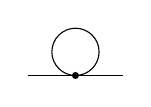
\begin{tikzpicture}[scale=0.3, baseline]

      \coordinate (B) at (-2,-1);
      \coordinate (C) at (2,-1);
      \draw (B) -- (C);
      \draw (0,0) circle (1.0);
      \filldraw (0,-1) circle (3.5pt);
    \end{tikzpicture}%
  }
}

\begin{document}

\maketitle
\section{Intro to LFT – Exercise sheet 2 (2025-05-08)}
{
\color{blue}
In the following problems, \( A_\mu(x) \) is a smooth \( \mathrm{SU}(N) \) gauge field in Euclidean spacetime. In particular, this means that \( A_\mu(x) \) is an element of the Lie algebra \( \mathfrak{su}(N) \) associated to the Lie group \( \mathrm{SU}(N) \); that is, it is an \( N \times N \) traceless Hermitian matrix. Even though \( A_\mu(x) \) can be decomposed with respect to a basis of generators, you will not need such a representation.
\begin{itemize}
\item The field tensor is defined as:
\begin{equation}
F_{\mu\nu} = \partial_\mu A_\nu - \partial_\nu A_\mu + i [A_\mu, A_\nu].
\end{equation}
In particular \( F_{\mu\nu}(x) \) is also an element of the Lie algebra \( \mathfrak{su}(N) \).

\item A gauge transformation \( \Omega(x) \) is an element of the gauge group \( \mathrm{SU}(N) \). Under a gauge transformation, the gauge field transforms as:
\begin{equation}
A_\mu \rightarrow A_\mu^{[\Omega]} = \Omega A_\mu \Omega^\dagger + i (\partial_\mu \Omega) \Omega^\dagger.
\end{equation}
\item Using the definition of the field tensor, one easily proves that under a gauge transformation:
\begin{equation}
F_{\mu\nu} \rightarrow F_{\mu\nu}^{[\Omega]} = \Omega F_{\mu\nu} \Omega^\dagger.
\end{equation}
\end{itemize}
}


\subsection{Exercise 1 - Path-ordered exponential}
{\color{blue}
Consider a smooth parametric curve $[s_0, s_1] \ni s \mapsto \gamma(s) \in \mathbb{R}^4$ in Euclidean spacetime. The following Cauchy problem:
\[
\begin{cases}
\displaystyle \frac{d}{ds} P(s) = i P(s) A_\mu(\gamma(s)) \gamma'^\mu(s), \\
P(s_0) = \mathbb{I}_N,
\end{cases}  \tag{4}
\]
where $P(s)$ is an $N \times N$ matrix, admits a unique solution for $s \in [s_0, s_1] $. The solution $P(s)$ is referred to as the \textit{path-ordered exponential} of the gauge field $A_\mu$ along the curve $\gamma$, and it is denoted by
\[
P(s) = \mathcal{P} \exp\left( i \int_{s_0}^s d\sigma\, \gamma'^\mu(\sigma) A_\mu(\gamma(\sigma)) \right). \tag{5}
\]
In particular, $P(s_1)$ is referred to as the \textit{parallel transport} along the curve $\gamma$, and it is often denoted by $W(\gamma)$. The following notation is also often used:
\[
W(\gamma) = \mathcal{P} \exp\left( i \int_{\gamma} dx^\mu A_\mu(x) \right). \tag{6}
\]
If $\gamma$ parametrizes a segment, then $W(\gamma)$ is referred to as the \textit{Wilson line} along $\gamma$. If $\gamma$ is a closed curve, then $W(\gamma)$ is referred to as the \textit{Wilson loop} along $\gamma$. We stress that the expressions given on the right-hand side of Eqs. (5) and (6) are just symbols, whose definition is given in terms of the solution of the Cauchy problem (4).

We now want to study some properties of the solution $P(s)$.
\begin{enumerate}[a.)]
\item \textbf{Special unitarity.} Using the Cauchy problem (4), prove that $P(s)$ is a special unitary matrix for every $s$, i.e., that
$P(s)P^\dagger(s) = \mathbb{I}_N \quad \text{and} \quad \det P(s) = 1.$

\textit{Hint:} Write differential equations for $P(s)P^\dagger(s)$ and $\det P(s)$, and solve them.
\item \textbf{Parametrization invariance.} Let $\tilde{\gamma}$ be a reparametrization of the curve $\gamma$, which preserves orientation. This is defined by providing an invertible function $[\tilde{s}_0, \tilde{s}_1] \ni \tilde{s} \mapsto h(\tilde{s}) \in [s_0, s_1]$, with the property that $ h(\tilde{s}_0) = s_0$ and $h(\tilde{s}_1) = s_1$. In terms of this function, we write
    \[
    \tilde{\gamma}(\tilde{s}) = \gamma(h(\tilde{s})). \tag{7}
    \]
    Let \( \tilde{P}(\tilde{s}) \) be the unique solution of the Cauchy problem
    \[
    \begin{cases}
    \displaystyle \frac{d}{d\tilde{s}} \tilde{P}(\tilde{s}) = i \tilde{P}(\tilde{s}) A_\mu(\tilde{\gamma}(\tilde{s})) \tilde{\gamma}'^\mu(\tilde{s}), \\
    \tilde{P}(\tilde{s}_0) = \mathbb{I}_N,
    \end{cases} \tag{8}
    \]
Prove that $\tilde{P}(\tilde{s}) = P(h(\tilde{s})).$

\textit{Note:} This equation expresses the fact that the path-ordered exponential does not depend on the particular parametrization chosen for the curve $\gamma$.

\textit{Hint:} Write the differential equation for $P(h(\tilde{s}))$ and compare it with the differential equation for $\tilde{P}(\tilde{s})$.
\item \textbf{Dependence on initial condition.} Given a generic $N \times N$ matrix $M$, let $R(s)$ be the unique solution of the Cauchy problem
    \[
    \begin{cases}
    \displaystyle \frac{d}{ds} R(s) = i R(s) A_\mu(\gamma(s)) \gamma'^\mu(s), \\
    R(s_0) = M,
    \end{cases} \tag{9}
    \]
    Prove that the solution of this equation is given by
    \[
    R(s) = M \, \mathcal{P} \exp \left( i \int_{s_0}^s d\sigma\, \gamma'^\mu(\sigma) A_\mu(\gamma(\sigma)) \right). \tag{10}
    \]
\textit{Hint:} Write the differential equation satisfied by the right-hand side of the above equation, and compare it with the differential equation for \( R(s) \).

\item \textbf{Group property.} Consider $s_0 \leq \bar{s} \leq s \leq s_1$. Prove that
    \[
    \mathcal{P} \exp \left( i \int_{s_0}^s d\sigma\, \gamma'^\mu(\sigma) A_\mu(\gamma(\sigma)) \right)
    =
    \mathcal{P} \exp \left( i \int_{s_0}^{\bar{s}} d\sigma\, \gamma'^\mu(\sigma) A_\mu(\gamma(\sigma)) \right)
    \cdot
    \mathcal{P} \exp \left( i \int_{\bar{s}}^{s} d\sigma\, \gamma'^\mu(\sigma) A_\mu(\gamma(\sigma)) \right).
    \tag{11}
    \]
Provide a geometrical interpretation of this equation.

\textit{Hint:} Show that both sides satisfy the same Cauchy problem.
\item \textbf{Gauge transformation.} Prove that
    \[
    \mathcal{P} \exp \left( i \int_{s_0}^s d\sigma\, \gamma'^\mu(\sigma) A_\mu^{[\Omega]}(\gamma(\sigma)) \right)
    =
    \Omega(\gamma(s_0))
    \cdot
    \mathcal{P} \exp \left( i \int_{s_0}^s d\sigma\, \gamma'^\mu(\sigma) A_\mu(\gamma(\sigma)) \right)
    \cdot
    \Omega^\dagger(\gamma(s)).
    \tag{12}
    \]
\textit{Hint:} Show that both sides of the above equation satisfy the same Cauchy problem.

\item \textbf{Approximation as product of exponentials.} Prove that, if $\Delta s$ is small,
    \[
    \mathcal{P} \exp \left( i \int_s^{s+\Delta s} d\sigma\, \gamma'^\mu(\sigma) A_\mu(\gamma(\sigma)) \right)
    =
    e^{i \gamma'^\mu(s) A_\mu(\gamma(s)) \Delta s} + \mathcal{O}(\Delta s^2).
    \tag{13}
    \]
    Use this fact to argue that the path-ordered exponential can be approximated by a product of standard exponentials of the gauge field, as in
    \[
    \mathcal{P} \exp \left( i \int_{s_0}^{s_1} d\sigma\, \gamma'^\mu(\sigma) A_\mu(\gamma(\sigma)) \right)
    =
    \lim_{N \to \infty}
    \prod_{k=0}^{N-1}
    e^{i \gamma'^\mu(\sigma_k) A_\mu(\gamma(\sigma_k)) \Delta \sigma},
    \tag{14}
    \]
    where
    \[
    \sigma_k = s_0 + k \Delta \sigma, \quad \Delta \sigma = \frac{s_1 - s_0}{N}.
    \tag{15}
    \]
\textit{Note:} A full proof of this fact is beyond the scope of this exercise sheet; a plausible argument is sufficient.
\end{enumerate}
}
\begin{enumerate}[a.)]
\item Using $\frac{d}{ds}P(s)$ and the fact that $A_\mu(\gamma(x))$ is hermitian (because SU($N$) matrix $e^{i\mathfrak{su}(2)}$ is unitary)
\begin{align}
\frac{d}{ds}P(s)P^\dagger(s)
&=\frac{dP(s)}{ds}P^\dagger(s)+P(s)\frac{dP^\dagger(s)}{ds}\\
&=[iP(s)A_\mu(\gamma(x))\gamma'^\mu(s)]P^\dagger(s)+P(s)[iP(s)A_\mu(\gamma(x))\gamma'^\mu(s)]^\dagger\\
&=iP(s)A_\mu(\gamma(x))\gamma'^\mu(s)P^\dagger(s)-iP(s)\gamma'^\mu(s)\underbrace{A^\dagger_\mu(\gamma(x))}_{=A_\mu(\gamma(x))}P^\dagger(s)\\
&=0
\end{align}
and the initial condition
\begin{align}
P(s_0)=\mathbb{I}_N
&\rightarrow P^\dagger(s_0)=\mathbb{I}\\
&\rightarrow P(s_0)P^\dagger(s_0)=\mathbb{I}
\end{align}
we conclude
\begin{align}
P(s)P^\dagger(s)=\mathbb{I}_N\qquad\forall s.
\end{align}
Now using the fact that $A_\mu$ is trace free
\begin{align}
1=\text{det\,SU}(N)=\text{det\,}e^{\mathfrak{su}(N)}=e^{\text{tr}(\mathfrak{su}(N))}\rightarrow\text{tr}(\mathfrak{su}(N))=0
\end{align}
and the Jacobi formula
\begin{align}
\frac{d}{ds}\text{det}P(s)
&=\text{det}P(s)\cdot\text{tr}\left(P^{-1}(s)\frac{dP(s)}{ds}\right)\\
&=\text{det}P(s)\cdot\text{tr}\left(P^{-1}(s)[iP(s)A_\mu(\gamma(x))\gamma'^\mu(s)]\right)\\
&=i\;\gamma'^\mu(s)\text{det}P(s)\cdot\underbrace{\text{tr}\left(A_\mu(\gamma(x)) \right)}_{=0}\\
&=0
\end{align}
and the initial condition
\begin{align}
P(s_0)=\mathbb{I}_N
&\rightarrow \text{det}P(s_0)=1
\end{align}
to conclude that $\text{det}P(s)=1$
\item Initial conditions
\begin{align}
P(h(\tilde{s}_0))=P(s_0)
\end{align}
and the differential equation
\begin{align}
\frac{d}{d\tilde{s}}P(h(\tilde{s}))
&=\frac{dP(h(\tilde{s}))}{dh}\frac{dh}{d\tilde{s}}\\
&=i P(h) A_\mu(\gamma(h)) \underbrace{\underbrace{\gamma'^\mu(h)}_{=\frac{d\tilde{\gamma^\mu}}{dh}}\frac{dh}{d\tilde{s}}}_{=\frac{d\tilde{\gamma^\mu}}{d\tilde{s}}}\\
&=i P(h(\tilde{s})) A_\mu(\gamma(h(\tilde{s})))\frac{d\tilde{\gamma^\mu}}{d\tilde{s}}
\end{align}
so we see that the differential equations for $\tilde{P}(\tilde{s})$ and $P(h(\tilde{s}))$ are identical.
\item Using
\begin{align}
\frac{d}{ds}\int_{g(s)}^{h(s)}f(t,s)dt
&=\frac{d}{ds}\left(F[h(s),s]-F[g(s),s]\right)\\
&=\frac{\partial F}{\partial h}\frac{\partial h}{\partial s}+\frac{\partial F[h,s]}{\partial s}-\frac{\partial F}{\partial g}\frac{\partial g}{\partial s}-\frac{\partial F[g,s]}{\partial s}\\
&=f(h(s))h'(s) - f(g(s))g'(s)+\int_{g(s)}^{h(s)}\frac{d}{ds}f(t,s)dt
\end{align}
and substituting the solution into the differential equations 
\begin{align}
\frac{dR}{ds}
&=\frac{d}{ds}\,M\mathcal{P}\exp\left(i\int_{s_0}^s d\sigma\,\gamma'^{\mu}(\sigma)A_\mu(\gamma(\sigma))\right)\\
&=\underbrace{M\mathcal{P}\exp\left(i\int_{s_0}^s d\sigma\,\gamma'^{\mu}(s)A_\mu(\gamma(s))\right)}_{=R(s)}(i \gamma'^{\mu}(\sigma)A_\mu(\gamma(\sigma)))\frac{ds}{ds}\\
&=iR(s)A_\mu(\gamma(s))\gamma'^{\mu}(s)
\end{align} 
so we see the the solution obeys the differential equation.
\item LHS
\begin{align}
\frac{d}{ds}\mathcal{P}\exp\left(i\int_{s_0}^s d\sigma\,\gamma'^{\mu}(\sigma)A_\mu(\gamma(\sigma))\right)
&=\mathcal{P}\exp\left(i\int_{s_0}^s d\sigma\,\gamma'^{\mu}(\sigma)A_\mu(\gamma(\sigma))\right)iA_\mu(\gamma(s))\gamma'^{\mu}(s)\\
\rightarrow\qquad\frac{d}{ds}Q(s)
&=Q(s)\cdot iA_\mu(\gamma(s))\gamma'^{\mu}(s)
\end{align}
RHS
\begin{align}
\frac{d}{ds}\mathcal{P} \exp &\left( i \int_{s_0}^{\bar{s}} d\sigma\, \gamma'^\mu(\sigma) A_\mu(\gamma(\sigma)) \right)
\cdot
\mathcal{P} \exp \left( i \int_{\bar{s}}^{s} d\sigma\, \gamma'^\mu(\sigma) A_\mu(\gamma(\sigma)) \right)\\
&=\exp \left( i \int_{s_0}^{\bar{s}} d\sigma\, \gamma'^\mu(\sigma) A_\mu(\gamma(\sigma)) \right)
\cdot
\mathcal{P} \exp \left( i \int_{\bar{s}}^{s} d\sigma\, \gamma'^\mu(\sigma) A_\mu(\gamma(\sigma)) \right)iA_\mu(\gamma(s))\gamma'^{\mu}(s)\\
&\qquad\rightarrow\qquad\frac{d}{ds}Q(s)
=Q(s)\cdot iA_\mu(\gamma(s))\gamma'^{\mu}(s)
\end{align}
\item LHS
\begin{align}
\frac{d}{ds}\left(\mathcal{P}\exp\left(i\int_{s_0}^s d\sigma\,\gamma'^{\mu}(\sigma)A^{[\Omega]}_\mu(\gamma(\sigma))\right)\right)
&=\mathcal{P}\exp\left(i\int_{s_0}^s d\sigma\,\gamma'^{\mu}(\sigma)A^{[\Omega]}_\mu(\gamma(\sigma))\right)iA^{[\Omega]}_\mu(\gamma(s))\gamma'^{\mu}(s)
\end{align}
RHS with $A_\mu^{[\Omega]} = \Omega A_\mu \Omega^\dagger + i (\partial_\mu \Omega) \Omega^\dagger$ and the adjoint $A_\mu^{[\Omega]} = \Omega A_\mu \Omega^\dagger - i (\Omega\partial_\mu \Omega^\dagger) $
\begin{align}
\frac{d}{ds}&\left(\Omega(\gamma(s_0))
\cdot
\mathcal{P} \exp\left( i \int_{s_0}^s d\sigma\, \gamma'^\mu(\sigma) A_\mu(\gamma(\sigma)) \right)
\cdot
\Omega^\dagger(\gamma(s)) \right)\\
&=\Omega(\gamma(s_0))\left(\frac{d}{ds}\mathcal{P} \exp\left( i \int_{s_0}^s d\sigma\, \gamma'^\mu(\sigma) A_\mu(\gamma(\sigma)) \right)\right)\Omega^\dagger(\gamma(s))\\
&\qquad+\Omega(\gamma(s_0))\mathcal{P} \exp\left( i \int_{s_0}^s d\sigma\, \gamma'^\mu(\sigma) A_\mu(\gamma(\sigma)) \right)\left(\frac{d}{ds}\Omega^\dagger(\gamma(s))\right)\\
&=\Omega(\gamma(s_0))\mathcal{P} \exp\left( i \int_{s_0}^s d\sigma\, \gamma'^\mu(\sigma) A_\mu(\gamma(\sigma)) \right)\left(iA_\mu(\gamma(s))\gamma'^{\mu}(s)\right)\Omega^\dagger(\gamma(s))\\
&\qquad+\Omega(\gamma(s_0))\mathcal{P} \exp\left( i \int_{s_0}^s d\sigma\, \gamma'^\mu(\sigma) A_\mu(\gamma(\sigma)) \right)\underbrace{\left(\frac{d}{ds}\Omega^\dagger(\gamma(s))\right)}_{=\partial_\nu\Omega^\dagger\gamma'^\nu(s)}\\
&=\Omega(\gamma(s_0))\mathcal{P} \exp\left( i \int_{s_0}^s d\sigma\, \gamma'^\mu(\sigma) A_\mu(\gamma(\sigma)) \right)\left(iA_\mu(\gamma(s))\gamma'^{\mu}(s)\right)\Omega^\dagger(\gamma(s))\\
&\qquad+\Omega(\gamma(s_0))\mathcal{P} \exp\left( i \int_{s_0}^s d\sigma\, \gamma'^\mu(\sigma) A_\mu(\gamma(\sigma)) \right)\gamma'^\nu(s)\partial_\nu\Omega^\dagger\\
&=\Omega(\gamma(s_0))\mathcal{P} \exp\left( i \int_{s_0}^s d\sigma\, \gamma'^\mu(\sigma)A(\gamma^{\mu}(s))\right)\gamma'^\mu(\sigma)\underbrace{\left[iA_\mu(\gamma(s))\Omega^\dagger(\gamma(a))+\partial_\mu\Omega^\dagger\right]}_{=i\Omega^\dagger(\gamma(s)) A_\mu^{[\Omega]}}\\
&=\Omega(\gamma(s_0))\mathcal{P} \exp\left( i \int_{s_0}^s d\sigma\, \gamma'^\mu(\sigma)A_\mu(\gamma'^{\mu}(\sigma))\right)\Omega^\dagger(\gamma(s)) i\gamma'^\mu(s)A_\mu^{[\Omega]}
\end{align}
and therefore comparing LHS and RHS
\begin{align}
\mathcal{P} \exp\left( i \int_{s_0}^s d\sigma\, \gamma'^\mu(\sigma)A^{[\Omega]}_\mu(\gamma'^{\mu}(s))\right)=\Omega(\gamma(s_0))\mathcal{P} \exp\left( i \int_{s_0}^s d\sigma\, \gamma'^\mu(\sigma)A_\mu(\gamma'^{\mu}(s))\right)\Omega^\dagger(\gamma(s))
\end{align}
\item With $\gamma'^\mu(\sigma)A_\mu(\gamma'^{\mu}(\sigma)) =\gamma'^\mu(s)A_\mu(\gamma'^{\mu}(s))$ and the fact that the path-ordering becomes obsolete if the integrand it constant 
\begin{align}
\mathcal{P} \exp\left( i \int_{s}^{s+\Delta s} d\sigma\, \gamma'^\mu(\sigma)A_\mu(\gamma'^{\mu}(\sigma))\right)
&\simeq\mathcal{P} \exp\left( i \int_{s}^{s+\Delta s} d\sigma\, \gamma'^\mu(s)A_\mu(\gamma'^{\mu}(s))\right)\\
&\simeq \exp\left( i\,\gamma'^\mu(s)A_\mu(\gamma'^{\mu}(s))\int_{s}^{s+\Delta s} d\sigma\right)\\
&\simeq \exp\left( i\,\gamma'^\mu(s)A_\mu(\gamma'^{\mu}(s))\Delta s+\mathcal{O}(\Delta s^2)\right)
\end{align}
For the next part we use the group property (we showed above) - splitting this into $N$ equal sized sections $\Delta\sigma$
\begin{align}
\mathcal{P} &\exp\left( i \int_{s_0}^{s_1} d\sigma\, \gamma'^\mu(\sigma)A_\mu(\gamma'^{\mu}(\sigma))\right)\\
&=\mathcal{P} \exp\left( i \int_{s_0}^{s_0+\Delta \sigma} d\sigma\, \gamma'^\mu(\sigma)A_\mu(\gamma'^{\mu}(\sigma))\right)...\mathcal{P} \exp\left( i \int_{s_0+(N-1)\Delta\sigma}^{s_1} d\sigma\, \gamma'^\mu(\sigma)A_\mu(\gamma'^{\mu}(\sigma))\right)\\
&\simeq\lim_{N\rightarrow\infty} \exp\left( i\,\gamma'^\mu(s_0)A_\mu(\gamma'^{\mu}(s_0))\Delta\sigma\right)...\exp\left( i\,\gamma'^\mu(s_0+(N-1)\Delta\sigma)A_\mu(\gamma'^{\mu}(s_0+(N-1)\Delta\sigma))\Delta\sigma\right)\\
&\simeq\lim_{N\rightarrow\infty} \exp\left( i\,\gamma'^\mu(s_0)A_\mu(\gamma'^{\mu}(s_0))\Delta\sigma\right)...\exp\left( i\,\gamma'^\mu(s_{N-1})A_\mu(\gamma'^{\mu}(s_{N-1})\Delta\sigma\right)
\end{align}
I think the limit is the handwavy part. 
\end{enumerate}

\subsection{Exercise 2 - Temporal gauge}
{\color{blue}
Given a gauge field $A_\mu(x)$, prove that it is always possible to find a gauge transformation $\Omega(x)$ such that $A^{[\Omega]}_0(x)=0$ for every $x$ (temporal gauge condition). Derive a formula for $\Omega(x)$ in terms of the path-ordered exponential.
}

We require (using $\Omega^{-1}=\Omega^\dagger$)
\begin{align}
A_0^{[\Omega]} 
&= \Omega A_0 \Omega^\dagger + i (\partial_0 \Omega) \Omega^\dagger\overset{!}{=}0\\
&\rightarrow  \Omega A_0 + i(\partial_0 \Omega)=0\\
&\rightarrow  \partial_0 \Omega=i\Omega A_0(\vec{x},t)
\end{align}
so we obtained a homogeneous linear first order ODE which we can solve as usual by separation of variables
\begin{align}
\Omega(\vec{x},t)=\mathcal{P}\exp\left(i\int_{t_0}^t A_0(\vec{x},s) ds\right)
\end{align}

\newpage
\section{Intro to LFT – Exercise sheet 1 (2025-04-15)}
\subsection{Exercise 1 - Integration of scalar function over multidimensional vector space}
Since the new basis $\{b^n\}$ needs to be orthonormal - the allowed transformations are
\begin{enumerate}
\item permutation of the basis vectors $\{e^n\}$
\item and then a rigid rotation of the whole basis  
\end{enumerate}
This transformations of the basis mean ($O\in O(N)$)
\begin{align}
e^n&=\sum_mO^n_{\,m}b^m\\
\rightarrow v&=\alpha_n e^n\\
&=\sum_m(\sum_n O^n_{\,m}\alpha_n) b^m\\
&=\sum_m\beta_m b^m\\
\rightarrow \beta_m&=\sum_n O^n_{\,m}\alpha_n
\end{align}
Now with $d\beta_m=\sum_n O^n_{\,m}d\alpha_n$
\begin{align}
I'(f)
&=\int\left(\prod_i d\beta_i\right)  f(\underbrace{\beta_k b^k}_{=\alpha_k a^k})\\
&=\int\left(\prod_i \sum_n O^n_{\,i}d\alpha_n\right)  f(\underbrace{\beta_k b^k}_{=\alpha_k a^k})\\
&=\int |\underbrace{\det O}_{\pm1}|\left(\prod_i d\alpha_n\right)  f(\underbrace{\beta_k b^k}_{=\alpha_k a^k})\\
&=\int \left(\prod_i d\alpha_n\right)  f(\alpha_k a^k)\\
&=I(f)
\end{align}

\newpage
\subsection{Exercise 2 - Multivariate Gaussian integral with a source}
As usual we try to obtain a complete square
\begin{align}
-\frac{1}{2}\phi^TA\phi+J^T\phi
&=-\frac{1}{2}\left(\phi^TA\phi-2J^T\phi\right)\\
&=-\frac{1}{2}\left((\phi+x)^TA(\phi+x)\right)+y\\
&=-\frac{1}{2}\left(\phi^TA\phi+\phi^TAx+x^TA\phi+x^TAx\right)+y
\end{align}
with $x=-A^{-1}J$
\begin{align}
-\frac{1}{2}\phi^TA\phi+J^T\phi
&=-\frac{1}{2}\left(\phi^TA\phi-\phi^TA(A^{-1}J)-(A^{-1}J)^TA\phi+(A^{-1}J)^TA(A^{-1}J)\right)+y\\
&=-\frac{1}{2}\left(\phi^TA\phi-J^T\phi+\phi^TJ+J^TA^{-1}J\right)+\frac{1}{2}J^TA^{-1}J\\
&=-\frac{1}{2}\left(\phi^TA\phi-J^T\phi+(J^T\phi)^T+J^TA^{-1}J\right)+\frac{1}{2}J^TA^{-1}J\
\end{align}
and therefore
\begin{align}
-\frac{1}{2}\phi^TA\phi+J^T\phi
&=-\frac{1}{2}(\phi-A^{-1}J)^TA(\phi-A^{-1}J)+\frac{1}{2}J^TA^{-1}J
\end{align}
So
\begin{align}
I(J)&=\int d\phi\; \exp\left[-\frac{1}{2}(\phi-A^{-1}J)^TA(\phi-A^{-1}J)\right]\cdot\exp\left[\frac{1}{2}J^TA^{-1}J\right]\\
&=\exp\left[\frac{1}{2}J^TA^{-1}J\right]\cdot\int d\phi\; \exp\left[-\frac{1}{2}(\phi-A^{-1}J)^TA(\phi-A^{-1}J)\right]
\end{align}
To calculate the remaining integral will now try to break it into a product of 1d gaussian integrals (which we know how to calculate).
\begin{itemize}
\item As $A$ is real and symmetric we can write it as $A=S^TDS$ where $D$ is diagonal (with positive eigenvalues of $A$ on the diagonal) and $S$ is orthogonal $S^{-1}=S^T$
\begin{align}
I(0)
&=\int d\phi\; \exp\left[-\frac{1}{2}(\phi-A^{-1}J)^T S^TDS (\phi-A^{-1}J)\right]\\
&=\int d\phi\; \exp\left[-\frac{1}{2}[S(\phi-A^{-1}J)]^T D [S(\phi-A^{-1}J)]\right]\\
&=\int d\phi\; \prod_k\exp\left[-\frac{1}{2}[S(\phi-A^{-1}J)]_k^T D_{kk} [S(\phi-A^{-1}J)]_k\right]
\end{align}
\item Now we can use the result of problem 1 - getting a new orthogonal coordinate system
\begin{align}
I(0)
&=\int d\phi\; \prod_k\exp\left[-\frac{1}{2}[S(\phi-A^{-1}J)]_k^T D_{kk} [S(\phi-A^{-1}J)]_k\right]\\
&=\prod_k\int d\psi_k\; \exp\left[-\frac{1}{2}\psi_k^T D_{kk} \psi_k\right]\\
&=\prod_k\sqrt{\frac{2\pi}{D_{kk}}}\\
&=\sqrt{\frac{(2\pi)^N}{det A}}
\end{align}
\end{itemize} 
And therefore
\begin{align}
I(J)&=\frac{(2\pi)^{N/2}}{\sqrt{\det A}}\exp\left[\frac{1}{2}J^TA^{-1}J\right]
\end{align}
which is finite for every $J$.

\newpage
\subsection{Exercise 3}
With
\begin{align}
(A\phi)_n&=\frac{2\phi_n-\phi_{n\oplus(+1)}-\phi_{n\oplus(-1)}}{a^2}\qquad(n=1,...,N)
\end{align}
we see that $A$ is the 1d negative discretized Laplacian with periodic boundary conditions (know from finite difference numerics of the heat and Schroedinger equation)
\begin{align}
A&=\frac{1}{a^2}\left(
\begin{matrix}
 2 & -1 &  0 &...& 0 & 0 & -1\\
-1 &  2 & -1 &...& 0 & 0 &  0\\
 0 & - 1&  2 &...& 0 & 0 &  0 \\
\vdots & & & & & &\vdots \\
 0 & 0 &  0 &...& 2 &-1 & 0\\
 0 & 0 &  0 &...&-1 & 2 &-1\\
-1 & 0 &  0 &...& 0 &-1 & 2\\
\end{matrix}
\right)
\end{align}
This looks like the set of equations of motion for a 1D chain of atoms
\begin{align}
m\ddot{x}_i=k(u_{i-1}-u_i)+k(u_{i+1}-u_i)
\end{align}
in matrix form.
\begin{enumerate}[1.]
\item We see that $A$ is symmetric -  $A$ is positive definite if and only if all eigenvalues are strictly positive - which we might see - once we calculated the eigenvalues.

\item The periodic boundary conditions imply
\begin{align}
v^{(p)}_0=v^{(p)}_N
&\quad\rightarrow\quad e^{iapN}=1\\
&\quad\rightarrow\quad apN=2\pi k\qquad(k\in\{1,2,3,...,N\})\\
&\quad\rightarrow\quad p=\frac{2\pi k}{aN}\qquad(\text{Nyquist-Shannon-sampling theorem})
\end{align}
and with $e^{iapN}=1$ we can calculate
\begin{align}
(Av^{(p)})_n
&=(Ae^{iapn})_n\\
&=\begin{cases}
\frac{1}{a^2}(2e^{iap\cdot1}-e^{iap\cdot2}-e^{iapN})=\frac{1}{a^2}(2-e^{iap}-e^{-iap})e^{iap}\qquad(n=1)\\
\frac{1}{a^2}(2e^{iapn}-e^{iap(n+1)}-e^{iap(n-1)})=\frac{1}{a^2}(2-e^{iap}-e^{-iap})e^{iapn}\qquad\text{else}\\
\frac{1}{a^2}(2e^{iapN}-e^{iap\cdot(1)}-e^{iap\cdot(N-1)})=\frac{1}{a^2}(2-e^{iap}-e^{-iap})e^{iapN}\qquad(n=N)
\end{cases}\\
&=\frac{1}{a^2}(2-e^{iap}-e^{-iap})v^{(p)}_n\\
&=\frac{2}{a^2}(1-\cos ap)v^{(p)}_n
\end{align}
Now we can read-off the $N$ eigenvectors and eigenvalues are ($1\le k\le N$)
\begin{align}
v^{(k)}_n
&=e^{ian\frac{2\pi k}{aN}}
=e^{2\pi i\frac{n}{N}k}\\
\lambda^{(k)}
&=\frac{2}{a^2}\left(1-\cos a\frac{2\pi k}{aN}\right)\\
&=\frac{2}{a^2}\left(1-\cos \frac{2\pi k}{N}\right)\\
&=\frac{2}{a^2}\left(1-\cos^2 \frac{\pi k}{N}+\sin^2 \frac{\pi k}{N}\right)\\
&=\frac{4}{a^2}\sin^2 \frac{\pi k}{N}=\left(\frac{2}{a}\sin\frac{\pi k}{N}\right)^2
\end{align}
As expected - this looks like the dispersion relation $\omega(k)$ for a 1D chain of atoms.
Now we see that $\lambda^{(N)}=0$ so $A$ is NOT positive definite but positive semi-definite.

\item Lets rewright
\begin{align}
v^{(k)}
&=e^{2\pi i\frac{n}{N}k}=\cos\left(2\pi\frac{n}{N}k\right)+i\sin\left(2\pi\frac{n}{N}k\right)
\end{align}
so - using results from elementary Fourier analysis - we rewrite the completeness relation  as a (finite) Fourier series
\begin{center}
\begin{table}[!h]
\centering
\begin{tabular}{cllll}
\hline\hline
$k$ & $\lambda^{(k)}$ & \text{(complex\;)} $v^{(k)}_n$ & \text{(real\;)} $u^{(k)}_n$ & \text{(real\;)} $u^{(k)}_n$\\ \hline\hline
1 & $\frac{4}{a^2}\sin^2\left(\pi\frac{1}{N}\right)$ & $\exp\left(2\pi\frac{ in}{N}\right)$  & $\sqrt{\frac{2}{N}}\cos\left(2\pi\frac{n}{N}\right)$ & $\sqrt{\frac{2}{N}}\sin\left(2\pi \frac{n}{N}\right)$\\
2 & $\frac{4}{a^2}\sin^2\left(\pi\frac{2}{N}\right)$ & $\exp\left(2\pi\frac{2in}{N}\right)$  & $\sqrt{\frac{2}{N}}\cos\left(2\pi\frac{2n}{N}\right)$ & $\sqrt{\frac{2}{N}}\sin\left(2\pi \frac{2n}{N}\right)$\\
...\\
$(N/2)$ & $\frac{4}{a^2}$ & $\exp\left(i\pi n\right)$ & $\sqrt{\frac{2}{L}}(-1)^n$  & 0 \\
...\\
$N-2$ & 
$\frac{4}{a^2}\sin^2\left(\pi\frac{2}{N}\right)$ &
$\exp\left(-2\pi\frac{2in}{N}\right)$  & 
$\sqrt{\frac{2}{N}}\cos\left(2\pi\frac{2n}{N}\right)$ & 
$-\sqrt{\frac{2}{N}}\sin\left(2\pi \frac{2n}{N}\right)$\\
$N-1$ & 
$\frac{4}{a^2}\sin^2\left(\pi\frac{1}{N}\right)$ &
$\exp\left(-2\pi\frac{in}{N}\right)$  & 
$\sqrt{\frac{2}{N}}\cos\left(2\pi\frac{n}{N}\right)$ & 
$-\sqrt{\frac{2}{N}}\sin\left(2\pi \frac{n}{N}\right)$\\
$N$ & 
$0$ &
$1$  & 
$\sqrt{\frac{1}{N}}$ & 
$0$
\end{tabular}
\caption{Overview of eigensystems}
\end{table}
\end{center}
and we see that we can drop half of the sine and cosine eigenfunctions occurring twice (up to a potential sign) - so we can drop them. 
So depending on $N$ even or odd
\begin{align}
u^{(N)}&=\sqrt{\frac{1}{N}}\\
u^{(k)}&=\sqrt{\frac{2}{N}}\cos\left(2\pi\frac{n}{N}k\right)\qquad{(k=1..[N-1/2]})\\
u^{(N/2+k)}&=\sqrt{\frac{2}{N}}\sin\left(2\pi\frac{n}{N}k\right)\qquad{(k=1..[N-1/2]})\\
u^{(N/2)}&=\sqrt{\frac{2}{N}}(-1)^n\qquad\text{(iff $N$ is even)}
\end{align}
It looks a bit messy in the write-up but I think its clear.


\item The eigenvalues $\tilde\lambda^{(k)}$ of $A+m^2=A+1_{N\times N}m^2$ are 
\begin{align}
\tilde\lambda^{(k)}
&=\lambda^{(k)}+m^2\\
&=\frac{4}{a^2}\sin^2\frac{\pi k}{N}+m^2
\end{align}
while the eigenvectors are the same as for $A$. Using the spectral decomposition to calculate the inverse of $(A+m^2)^{-1}$ (which has the inverse eigenvalues and the same eigenvectors)
\begin{align}
(A+m^2)^{-1}&=\sum_k\frac{1}{\tilde\lambda^{(k)}}{u^{(k)}}^Tu^{(k)}\\
(A+m^2)^{-1}_{ij}&=\sum_k\frac{1}{\frac{4}{a^2}\sin^2\frac{\pi k}{N}+m^2}{u^{(k)}_i}^Tu^{(k)}_j
\end{align}
I tried to find a simple expression using Mathematica - but could not find anything.

Alternatively I also tried
\begin{align}
\frac{1}{A+m^2}&=\frac{1}{m^2}\left(1-\frac{1}{m^2}A+\frac{1}{m^4}A^2-\frac{1}{m^6}A^3+...\right)\\
\frac{1}{A+m^2}_{ij}
&={u^{(i)}}^T\frac{1}{A+m^2}{u^{(j)}}\\
&=\frac{1}{m^2}\left(1-\frac{1}{m^2}{u^{(i)}}^TA{u^{(j)}}+\frac{1}{m^4}{u^{(i)}}^TA^2{u^{(j)}}-\frac{1}{m^6}{u^{(i)}}^TA^3{u^{(j)}}+...\right)\\
&=\frac{1}{m^2}\left(1-\frac{1}{m^2}{u^{(i)}}^T\lambda^{(j)}{u^{(j)}}+\frac{1}{m^4}{u^{(i)}}^T(\lambda^{(j)})^2{u^{(j)}}-\frac{1}{m^6}{u^{(i)}}^T(\lambda^{(j)})^3{u^{(j)}}+...\right)\\
&=\frac{1}{m^2}\left(1
-\frac{\lambda^{(j)}}{m^2}{u^{(i)}}^T{u^{(j)}}
+\frac{(\lambda^{(j)})^2}{m^4}{u^{(i)}}^T{u^{(j)}}
-\frac{(\lambda^{(j)})^3}{m^6}{u^{(i)}}^T{u^{(j)}}+...\right)
\end{align}
but got nowhere.
\end{enumerate}

\newpage
\section{O(3) non-linear sigma model in two-dimension}
This is a theory with action (Euclidean metric $\eta=\text{diag}(+1,+1))$
\begin{align}
S
&=\frac{1}{2g^2}\int d^2x \sum_k \partial_\mu \phi_k\partial^\mu \phi_k\\
&=\frac{1}{2g^2}\int d^2x \sum_k |\partial_\mu \phi_k|^2
\end{align}
where the field had three components $\phi(x,y) = ( \phi_1(x,y), \phi_2(x,y), \phi_3(x,y) )$ and lives on a sphere with unit radius, i.e.
\begin{align}
\phi_1^2+\phi_2^2+\phi_3^2 &= 1
\end{align}

\subsection{Discretization of the field}
Assumption: cubic equidistant lattice ($a=a_x=a_y$)
\begin{align}
S&=\frac{1}{2g^2}\int dx\,dy (\partial_x\phi_1)^2+(\partial_x\phi_2)^2+(\partial_x\phi_3)^2+(\partial_y\phi_1)^2+(\partial_y\phi_2)^2+(\partial_y\phi_3)^2\\
&\simeq\frac{a^2}{2g^2}\sum_{ij}\sum_{k}\frac{(\phi^{(k)}_{i+1,j}-\phi^{(k)}_{i,j})^2}{a^2}+\frac{(\phi^{(k)}_{i,j+1}-\phi^{(k)}_{i,j})^2}{a^2}\\
&\simeq\frac{a^2}{2g^2}\sum_{ij}\sum_{k}
\frac{(\phi^{(k)}_{i+1,j})^2}{a^2}
+\frac{(\phi^{(k)}_{i,j})^2}{a^2}
+\frac{(\phi^{(k)}_{i,j+1})^2}{a^2}
+\frac{(\phi^{(k)}_{i,j})^2}{a^2}
-2\frac{\phi^{(k)}_{i+1,j}\phi^{(k)}_{i,j}}{a^2}
-2\frac{\phi^{(k)}_{i,j+1}\phi^{(k)}_{i,j}}{a^2}\\
&\simeq
\frac{a^2}{2g^2}\sum_{ij}\frac{4}{a^2}
-\frac{a^2}{g^2}\sum_{k}\sum_{ij}
\frac{\phi^{(k)}_{i+1,j}\phi^{(k)}_{i,j}}{a^2}
+\frac{\phi^{(k)}_{i,j+1}\phi^{(k)}_{i,j}}{a^2}\\
&\simeq
\frac{2N_s^2}{g^2}
-\frac{1}{g^2}\sum_{k}\sum_{ij}
\phi^{(k)}_{i+1,j}\phi^{(k)}_{i,j}
+\phi^{(k)}_{i,j+1}\phi^{(k)}_{i,j}
\end{align}
we neglect the first term (constant offset) and use
\begin{align}
S_{ij}
&=-\frac{1}{g^2}\sum_{k}
\phi^{(k)}_{i+1,j}\phi^{(k)}_{i,j}
+\phi^{(k)}_{i,j+1}\phi^{(k)}_{i,j}\\
S_\text{tot}
&=\sum_{ij}S_{ij}\\
&=-\frac{1}{g^2}\sum_{k}\sum_{ij}
\phi^{(k)}_{i+1,j}\phi^{(k)}_{i,j}
+\phi^{(k)}_{i,j+1}\phi^{(k)}_{i,j}
\end{align}

\begin{align}
Z
&=\int d\phi_1d\phi_2d\phi_3\exp\left[-\frac{1}{2g^2}\int dx\,dy \sum_{k,\mu}|\partial_\mu\phi_k|^2\right]\\
&=\sum_\text{configs}\exp{[-S_\text{tot}(\phi^{(k)}_{i,j})]}\\
\langle\phi(x_1)\phi(x_2)\rangle
&=\frac{\int d\phi^{(1)}d\phi^{(2)}\phi^{(3)}\;\sum_{k'}\phi^{(k')}(x_1)\phi^{(k')}(x_2)\exp\left[-\frac{1}{2g^2}\int dx\,dy \sum_{k,\mu}|\partial_\mu\phi^{(k)}|^2\right]}
{\int d\phi^{(1)}d\phi^{(2)}\phi^{(3)}\;\exp\left[-\frac{1}{2g^2}\int dx\,dy \sum_{k,\mu}|\partial_\mu\phi^{(k)}|^2\right]}\\
C_{r_j}&=\frac{\sum_\text{configs}\frac{1}{N_{r_j}}\left(\sum_k\phi^{(k)}\phi^{(k)}\right)\exp{[-S_\text{tot}(\phi^{(k)}_{i,j})]}}{\sum_\text{configs}\exp{[-S_\text{tot}(\phi^{(k)}_{i,j})]}}
\end{align}

\subsection{Random field configuration at lattice point}
To generate a random field at a point of the lattice - obeying the $O(3)$ constraint we use polar coordinates. As the field vectors should be uniformly distributed in $S^2$ we use the uniformly independent distributed angle $\varphi\in[0,2\pi)$ and $z=\cos\vartheta\in[-1,+1)$
\begin{align}
\varphi   &= 2\pi\,\mathcal{U}^{(1)}_{[0,1]}\\
z=\cos\vartheta &= 2\,\mathcal{U}^{(2)}_{[0,1]}-1\qquad\rightarrow\qquad\sin\vartheta=\sqrt{1-\cos^2\theta}\\
\rightarrow\phi^{(1)}&=\sin\vartheta\, \cos\varphi\\
\rightarrow\phi^{(2)}&=\sin\vartheta\, \sin\varphi\\
\rightarrow\phi^{(3)}&=\cos\vartheta
\end{align} 

\subsection{Code}
\begin{algorithm}[!h]
\caption{Metropolis Monte Carlo for O(3) nonlinear sigma model in 2D}
\begin{algorithmic}[1]
\STATE Assumption - cubic equidistant lattice
\STATE Initialize a $N_x \times N_y$ lattice with random unit vectors $\vec{\phi}_{i,j}=\phi^{(k)}_{i,j} \in \mathbb{S}^2$
\STATE Initialize a $N_x \times N_y$ lattice with local action $S_{i,j}$
\STATE Calculate total action $S_\text{tot}=\sum_{ij}S_{ij}$
\STATE Initialize $Z=0$ 
\STATE Initialize all 2-point observables $c_{r_k}=0$ with $r_k\in\left\{\sqrt{k_x^2+k_y^2},\; 0\le k_x\le\sfrac{N_x}{2}, 0\le k_y\le\sfrac{N_y}{2}\right\}$
\STATE Calculate count of distance occurrence $N_{r_j}$

\FOR{$\text{step} = 1$ to ${\text{stepMax}}$}
    %\FOR{$\text{step} = 1$ to $L \times L$}
        \STATE Choose a random site on lattice $(x,y)$
        \STATE Backup current field: $\vec{\phi}_{\text{old}} = \vec{\phi}_{x,y}$ and total action $S_\text{tot(old)}=S_\text{tot}$
        \STATE Propose new field: $\phi^{(k)}_{x,y} =$ random unit vector on the sphere
        \STATE Update local action $S_{ij}$ for the discretized action of this model we actually only need to update action at three points $S_{x,y},S_{x-1,y},S_{x,y-1}$
        \STATE recompute total action $S_\text{tot}$
        \STATE Compute energy difference: $\Delta S = S_\text{tot} - S_\text{tot(old)}$
        \IF{$\Delta S \leq 0$}
            \STATE Accept: $\vec{\phi}_{x,y}$
        \ELSE
            \STATE Draw $r \sim \mathcal{U}_{[0,1]}$
            \IF{$r < \exp(-\Delta S)$}
                \STATE Accept: $\vec{\phi}_{x,y}$
            \ELSE
                \STATE Reject: $\vec{\phi}_{x,y}=\vec{\phi}_\text{old}$
            \ENDIF
        \ENDIF
    %\ENDFOR
    \IF{$\text{step} > \text{stepMin}$}
    	\STATE $Z=Z+\exp(-S_\text{tot})$
    	\FOR{all possible lattice distances $r_j=\sqrt{(x_1-x_2)^2+(y_1-y_2)^2}$}
    		\STATE $c_{r_j}=c_{r_j}+\frac{1}{N_{r_j}}\sum_{|p_1-p_2|=r_j}\left(\sum_k\phi^{(k)}_{j_{x1},j_{y1}}\phi^{(k)}_{j_{x2},j_{y2}}\right)\exp(-S_\text{tot})$
    	\ENDFOR
    \ENDIF
\ENDFOR
\STATE Calculate $C_{r_j}=\frac{c_{r_j}}{Z}$
\end{algorithmic}
\end{algorithm}

\subsection{First results}

\begin{figure}[!h]
\centering
%\includegraphics[width=0.40\textwidth]{/Users/christiant/MyDocuments/Programming/C/SigmaO3/convergence_1e-3.jpeg}
%\includegraphics[width=0.40\textwidth]{/Users/christiant/MyDocuments/Programming/C/SigmaO3/convergence_1e-2.jpeg}
\includegraphics[width=0.40\textwidth]{/Users/christiant/MyDocuments/Programming/C/SigmaO3/convergence_1e-1.jpeg}
\includegraphics[width=0.40\textwidth]{/Users/christiant/MyDocuments/Programming/C/SigmaO3/convergence_2e-1.jpeg}
\includegraphics[width=0.40\textwidth]{/Users/christiant/MyDocuments/Programming/C/SigmaO3/convergence_4e-1.jpeg}
\includegraphics[width=0.40\textwidth]{/Users/christiant/MyDocuments/Programming/C/SigmaO3/convergence_6e-1.jpeg}
\includegraphics[width=0.40\textwidth]{/Users/christiant/MyDocuments/Programming/C/SigmaO3/convergence_8e-1.jpeg}
\includegraphics[width=0.40\textwidth]{/Users/christiant/MyDocuments/Programming/C/SigmaO3/convergence_1e-0.jpeg}
\includegraphics[width=0.40\textwidth]{/Users/christiant/MyDocuments/Programming/C/SigmaO3/convergence_12e-0.jpeg}
\includegraphics[width=0.40\textwidth]{/Users/christiant/MyDocuments/Programming/C/SigmaO3/convergence_14e-0.jpeg}
\includegraphics[width=0.40\textwidth]{/Users/christiant/MyDocuments/Programming/C/SigmaO3/convergence_18e-0.jpeg}
\includegraphics[width=0.40\textwidth]{/Users/christiant/MyDocuments/Programming/C/SigmaO3/convergence_22e-0.jpeg}
\caption{convergence of $g^2S_\text{tot}/(N_x\times N_y)$ for various $g$ and various lattice sizes.}
\label{fig:example}
\end{figure}

\begin{figure}[!h]
\centering
\includegraphics[width=0.85\textwidth]{/Users/christiant/MyDocuments/Programming/C/SigmaO3/convergence.jpeg}

\caption{Mean and standard deviation of $g^2S_\text{tot}/(N_x\times N_y)$ at equilibrium (samplesize 1,000 after $10^7$ steps) for various $g$ for lattice size ($30\times30$)}
\label{fig:example1}
\end{figure}


\subsection{Extract mass gap from  $C(r)$}

\begin{align}
C(r)&=f(r)e^{-mr}\\
\rightarrow&\log\frac{C(r)}{C(r+1)}=\log\frac{f(r)e^{-mr}}{f(r)e^{-mr}e^{-m}}=m
\end{align}

%\begin{align}
%\frac{\left(\frac{8}{e}\right)^{\frac{1}{N-2}}}{\Gamma
%   \left(1+\frac{1}{N-2}\right)}\Lambda_{MS}
%\end{align}
%$\frac{8}{e}\Lambda_{MS}$, $\sqrt{\frac{32}{\pi e}}\Lambda_{MS}$


\newpage
\newpage
\section{Lectures}

\subsection{What is lattice field theory and why is it interesting}
\begin{enumerate}
\item LFT is Quantum Field Theory
\item If you calculate 1-loop Feynman diagrams you can see that they are UV divergent
\item example: $\phi^4$ theory
\begin{align}
\feynOneLoopConnect\quad\simeq
&\int\frac{d^4p}{(2\pi)^4}\frac{1}{p_0^2-\vec{p}^2-m^2+i\epsilon}\\
&\overset{\text{Wick rotation}}{\longrightarrow}\int\frac{d^4p}{(2\pi)^4}\frac{1}{p_0^2+\vec{p}^2+m^2}
=\int\frac{d^4p}{(2\pi)^4}\frac{1}{p^2+m^2}\sim\int_0^\infty dp\,p^3 \frac{1}{p^2}\rightarrow +\infty
\end{align}
\item In QFT you need to regularize UV divergencies (i.e. introduce a UV cut-off/regulator)
\item There are multiple ways to do this:
\begin{enumerate}
\item Hard cutoff ($\Lambda$ called UV regulator)
\begin{align}
\int_{|p|<\Lambda} \frac{d^4p}{(2\pi)^4}\frac{1}{p^2+m^2}
\end{align}
allowed momentum space is a sphere
\item Heat kernel regularization
\begin{align}
\int\frac{d^4p}{(2\pi)^4}\frac{e^{-p^2/\Lambda^2}}{p^2+m^2}
\end{align}
\item Dimensional regularization -  $D$ generic number of dimensions
\begin{align}
\int\frac{d^Dp}{(2\pi)^D}\frac{1}{p^2+m^2}
&\simeq\int_0^\infty p^{D-1}\frac{1}{p^2+m^2}\\
&\simeq\int_0^\infty p^{D-3}
\end{align}
UV convergent for $D=4-2\epsilon,\;(\epsilon>1)$, so for $\epsilon$ large enough the loop diagrams become UV finite.
\item The lattice is just another UV regulator
\begin{align}
\int \frac{d^4p}{(2\pi)^4}\frac{1}{p^2+m^2}
\qquad&\rightarrow\qquad\int_{-\pi/a}^{+\pi/a} \frac{d^4p}{(2\pi)^4}\frac{1}{\sum_\mu \left(\frac{2}{a}\sin\frac{p_\mu a}{2}\right)^2+m^2}\\
\qquad&\rightarrow\qquad\lim_{a\rightarrow 0 }\int_{-\pi/a}^{+\pi/a} \frac{d^4p}{(2\pi)^4}\frac{1}{\sum_\mu \left(\frac{2}{a}\frac{p_\mu a}{2}\right)^2+m^2}
\end{align}
the lattice constant $a$ is the UV regulator $-\frac{\pi}{a}\le p_\mu\le+\frac{\pi}{a}$. Again hard momentum cut-off $\Lambda=\pi/a$ (but here allowed momentum space is a cube not a sphere)
\end{enumerate}
\item Why is it interesting to consider the lattice regulator - isn't it just another hard cutoff?
\begin{enumerate}
\item Let's say that we are interested in QCD (theory that describes quarks and gluons)
\item QCD is a non-abelian gauge theory
\item Hard spherical cut-off and heat kernel regulatization break non-abelian gauge symmetry - so they are not suitable to study QCD
\item The only known regulators that do not break non-abelian gauge symmetry are dimensional and lattice regularization (maybe there are others?!)
\item However dimensional regularization is defined only in conjunction with the  perturbative expansion
\item QCD is supposed to be defined beyond perturbation theory - meaning in a non-perturbative sense
\begin{itemize}
\item Simplified universe: only gluons and the up and down quarks (which are massless, in reality their mass is very small)
\item then at any order of perturbation theory the mass of the proton is always zero
\item so the proton mass is essentially a non-perturbative observable
\end{itemize}
\item The lattice regulator is the only known regulator that allows to study QCD at the non-perturbative level
\begin{itemize}
\item due to running coupling constant (small at high energy, large at small energies $\sim1$GeV) - perturbation theory works well at high energies and non-perturbative methods need be used at low energies
\end{itemize}
\end{enumerate}
\end{enumerate}



\subsection{What does is mean to regularize QFT on a lattice?}

\subsubsection{Example: $\phi^4$-theory - Path integral formulation}
\begin{itemize}
\item Action in Minkowski spacetime $\eta=\text{diag}(1,\textcolor{red}{\bf-1},\textcolor{red}{\bf-1},\textcolor{red}{\bf-1})$: 
\begin{align}
S_\text{Minkowski}&=\int d^4x\left\{\frac{1}{2}\partial_\mu\phi(x)\partial^\mu\phi(x)-\frac{m^2}{2}\phi(x)^2-\frac{\lambda}{4!}\phi(x)^4\right\}\\
\mathcal{Z}&=\int \mathcal{D}\phi\; e^{iS_\text{M}(\phi)}
\end{align}
\item Expectation values are then defined by
\begin{align}
\langle P(\phi)\rangle =\frac{1}{\mathcal{Z}}\int \mathcal{D}\phi\; e^{iS_\text{M}}P(\phi)
\end{align}
with $\mathcal{D}\phi$ integral over all field configurations, $1/\mathcal{Z}$ normalization  and e.g. $P(\phi)=\phi(x)\phi(y)$.
\item One can alternatively define an action in Euclidean spacetime $\eta=\text{diag}(1,\textcolor{blue}{\bf+1},\textcolor{blue}{\bf+1},\textcolor{blue}{\bf+1})$: 
\begin{align}
S_\text{Euclid}&=\int d^4x\left\{\frac{1}{2}\partial_\mu\phi(x)\partial^\mu\phi(x)+\frac{m^2}{2}\phi(x)^2+\frac{\lambda}{4!}\phi(x)^4\right\}\\
\mathcal{Z}&=\int \mathcal{D}\phi\; e^{-S_\text{E}(\phi)}
\end{align}
\end{itemize}
\subsubsection*{Why Euclidean?}
\begin{enumerate}[(a)]
\item Minkowski $n$-point functions $\langle\phi(x_1)...\phi(x_2)\rangle_\text{M}$ can be obtained from Euclidean $n$-point functions $\langle\phi(x_1)...\phi(x_2)\rangle_\text{E}$ by analytically continuing in the time coordinates
\begin{align}
(x^{(E)}_k)_0=i(x^{(M)}_k)_0\qquad(\text{Wick rotation})
\end{align}
Euclidean \& Minkowski QFT contain the same information - one can go from one to the other using the Wick rotation
\item The lattice regulator for QFT only truly works in Euclidean space 
\end{enumerate}

\subsubsection*{General algorithm}
\begin{enumerate}[(1)]
\item Consider QFT in Euclidean
\item Regulate using the lattice
\item Calculate $n$-point functions
\item Remove the UV regulator: $a\rightarrow 0$ (after renormalization)
\item Wick rotate to Minkowskian
\end{enumerate}


\begin{center}
\begin{figure}[!h]
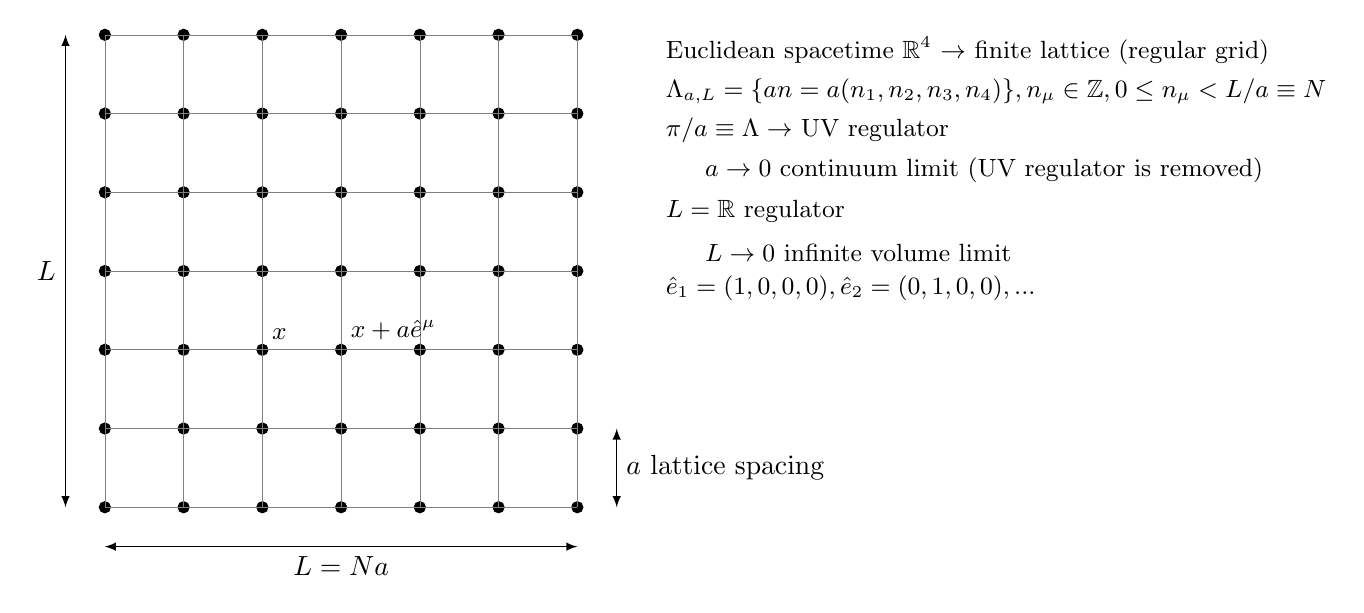
\begin{tikzpicture}
\def\L{6}
  % Draw the lattice points in a 5x5 grid
  \foreach \x in {0,...,\L}
    \foreach \y in {0,...,\L}
      \filldraw[black] (\x,\y) circle (2pt);
  
  % Optional: draw a grid
  \draw[step=1cm, gray, very thin] (0,0) grid (\L,\L);
  
    \draw[<->] (0,-0.5) -- (\L,-0.5) node[midway, below] {$L=Na$};
	\draw[<->] (-0.5,0) -- (-0.5,\L) node[midway, left] {$L$};
	\draw[<->] (\L+0.5,0) -- (\L+0.5,1) node[midway, right] {$a$ lattice spacing};
	
	\node[anchor=south west] at (2,2) {\small $x$};
	\node[anchor=south west] at (3,2) {\small $x+a\hat{e}^\mu$};
	
	\node[anchor=south west] at (\L+1,  \L-0.5) {\small Euclidean spacetime $\mathbb{R}^4$ $\rightarrow$ finite lattice (regular grid)};
	\node[anchor=south west] at (\L+1,  \L-1.0) {\small $\Lambda_{a,L}=\{an=a(n_1,n_2,n_3,n_4)\}, n_\mu\in\mathbb{Z}, 0\le n_\mu<L/a\equiv N$};
	\node[anchor=south west] at (\L+1,  \L-1.5) {\small $\pi/a\equiv\Lambda \rightarrow$ UV regulator};
	\node[anchor=south west] at (\L+1.5,\L-2.0) {\small $a\rightarrow0$ continuum limit (UV regulator is removed)};
	\node[anchor=south west] at (\L+1,  \L-2.5) {\small $L= \mathbb{R}$ regulator};
	\node[anchor=south west] at (\L+1.5,\L-3.0) {\small $L\rightarrow0$ infinite volume limit};
	\node[anchor=south west] at (\L+1,  \L-3.5) {\small $\hat{e}_1=(1,0,0,0), \hat{e}_2=(0,1,0,0), ...$};
	
\end{tikzpicture}
\end{figure}
\end{center}

\subsubsection*{Discretized Euclidean Action}
\begin{enumerate}[(1)]
\item The field $\phi(x)$ is only defined for $x\in \Lambda_{a,L}$ (on point that belongs to the lattice)
\item A (scalar) field configuration = field given at all points = one real number per lattice point = vector with $N^D$ components
\item Discretized forward derivative (not the only possible approximation)
\item $\mathcal{C}$ is the space of all field configurations - vector space $\simeq\mathbb{R}^{N^4}$
\begin{align}
\partial_\mu\phi(x)\rightarrow\hat{\partial}^f_\mu\phi(x)\equiv\frac{\phi(x+a\hat{e}_\mu)-\phi(x)}{a}
\end{align}
where $\hat{e}_\mu$ are the lattice unit vectors
\item In order to define $\partial^f_\mu$ on a finite lattice (at boundary lattice points $z=Na\hat{e}_\mu$) we need to specify boundary conditions
\begin{itemize}
\item Dirichlet boundary conditions: declare $\phi(z+a\hat{e}_1)\equiv0$
\item von Neumann boundary (periodic) conditions: declare $\phi(z+a\hat{e}_1)\equiv\phi(z+a\hat{e}_1-Na\hat{e}_1)$
\end{itemize}
\item Discretized integral (keep in mind Riemann sum approximation $\int_a^b dx f(x)\simeq\sum_{x_i}\Delta x\,f(x_i)$)
\begin{align}
\int d^4x\rightarrow\sum_{x\in\Lambda_{a,L}}a^4
\end{align}
then
\begin{align}
S_\text{E}
&=\int d^4x\left\{\frac{1}{2}\partial_\mu\phi(x)\partial^\mu\phi(x)+\frac{m^2}{2}\phi(x)^2+\frac{\lambda}{4!}\phi(x)^4\right\}\\
&=\sum_{x\in\Lambda_{a,N}}a^4\left\{\frac{1}{2}\sum_{\mu=1}^4\hat\partial^f_\mu\phi(x)\hat\partial^\mu\phi(x)+\frac{m^2}{2}\phi(x)^2+\frac{\lambda}{4!}\phi(x)^4\right\}
\end{align}
\item Using regularized path integral measure $\mathcal{D}\phi\equiv\prod_{x\in \Lambda_{a,N}}d\phi(x)$ so
\begin{align}
\int\mathcal{D}\phi=\int\underbrace{\prod_{x_k\in \Lambda_{a,N}}}_{
\begin{array}{c}
\scriptstyle \text{all points of} \\
\scriptstyle \text{the spactime lattice}
\end{array}
}\underbrace{ d\phi(x_k)}_{
\begin{array}{c}
\scriptstyle \text{integral over $\mathbb{R}$ } \\
\scriptstyle \text{(all field values $\phi$ at $x_k$)}
\end{array}
}
\end{align}
this are $N^4$ nested \textcolor{red}{\bf (NOT a product of) } integrals over $\mathbb{R}$ (one at each point of the lattice)
\item To calculate a meaningful expectation value
\begin{align}
\langle P(\phi)\rangle &=\frac{1}{\mathcal{Z}}\int \mathcal{D}\phi\; e^{iS_\text{M}}P(\phi)\\
\mathcal{Z}&=\int \mathcal{D}\phi\; e^{-S_\text{E}(\phi)}
\end{align}
we need the normalization to work so $\langle1\rangle=1$ which requires $\mathcal{Z}$ to be finite.

\item On a lattice on can prove
\begin{align}
\left|\int_\mathcal{C} \mathcal{D}\phi\; e^{-S_\text{E}(\phi)}P(\phi)\right|<+\infty
\end{align}
for each $P(\phi)$ which is polynomial in the field.

Proof for $P(1)$:
\begin{align}
S(\phi)&=\sum_{x\in\Lambda_{a,N}}a^4\left\{\frac{1}{2}\sum_{\mu=1}^4\hat\partial^f_\mu\phi(x)\hat\partial^\mu\phi(x)+\frac{m^2}{2}\phi(x)^2+\frac{\lambda}{4!}\phi(x)^4\right\}\\
&=\underbrace{\frac{1}{2}\sum_{x\in\Lambda}a^4\sum_{\mu=1}^4\left(\hat\partial^f_\mu\phi(x)\right)^2}_{\ge0}+
\underbrace{\frac{m^2}{2}\sum_{x\in\Lambda}a^4\phi(x)^2}_{\ge0}+
\underbrace{\frac{\lambda}{4!}\sum_{x\in\Lambda}a^4\phi(x)^4}_{\ge0}\\
&\ge \frac{m^2}{2}\sum_{x\in\Lambda}a^4\phi(x)^2\\
\rightarrow\; e^{-S(\phi)}&\le e^{-\frac{m^2}{2}\sum_{x\in\Lambda}a^4\phi(x)^2}\\
\rightarrow\; \mathcal{Z}&\le\int\mathcal{D}\phi\, e^{-\frac{m^2}{2}\sum_{x\in\Lambda}a^4\phi(x)^2}\\
&=\int\left\{\prod_{x_k\in\Lambda} d\phi(x_k)\right\}\, \prod_{x_j\in\Lambda} e^{-\frac{m^2}{2}a^4\phi(x_j)^2}
\end{align}
as the integrand a product of functions of the field at lattice points $\phi(x_k)$ the nested integrals separates to a product of integrals
\begin{align}
\mathcal{Z}&\le\prod_{x_k\in\Lambda}\int d\phi(x_k)\,e^{-\frac{m^2}{2}a^4\phi(x_k)^2}\\
&=\left(\int dz\;e^{-\frac{m^2a^4}{2}z^2}\right)^{N^4}\\
&=\left(\sqrt{\frac{2\pi}{m^2a^4}}\right)^{N^4}<\infty
\end{align}
\end{enumerate}

\subsection{QFT is Quantum Mechanics for Fields}
Hamiltonian for free scalar field
\begin{align}
H=\int\frac{d^3p}{(2\pi)^3}E(p)a^\dagger(p)a(p)\qquad\qquad E(p)=\sqrt{m^2+p^2}
\end{align}
derived from the standard classical field theoretical approach
\begin{align}
\mathcal{L}
&=\frac{1}{2}\partial_\mu\phi\partial^\mu\phi-\frac{m^2}{2}\phi^2-\frac{\lambda}{4!}\phi^4\\
&=\frac{1}{2}\partial_0\phi\partial^0\phi-\frac{1}{2}\partial_k\phi\partial^k\phi-\frac{m^2}{2}\phi^2-\frac{\lambda}{4!}\phi^4\\
&\qquad\qquad\rightarrow\pi(x)=\frac{\partial\mathcal{L}}{\partial(\partial_0\phi(x))}=\partial_0\phi(x)\\
\rightarrow L&=\int d^3x\,\mathcal{L}\\
\rightarrow H&=\left\{\frac{1}{2}\pi^2+\frac{1}{2}\partial_k\phi\partial^k\phi+\frac{m^2}{2}\phi^2+\frac{\lambda}{4!}\phi^4\right\}
\end{align}
Question: What is the connection between the path integral formalism and the canonical formalism?

\subsubsection{Quantum Mechanics Recap}

First: Lets consider the case of QM of the point particle in a generic number of dimensions:
\begin{itemize}
\item States $\equiv$ wave functions $\psi(q):\mathbb{R}^D\rightarrow\mathbb{C}$
\item Hilbert space $\mathcal{H}=\{\psi \text{ with } ||\psi||=\int d^Dq\,|\psi|^2<+\infty\}\equiv L^2(\mathbb{R}^2)$
\item Position operators $\hat{q}_k\psi(q)=q_k\psi(q)$ with $k=1,...,D$
\item Momentum operators $\hat{p}_k\psi(q)=-i\partial_{q_k}\psi(q)$
\item State $|\psi\rangle$
\begin{itemize}
\item Eigenstate of $\hat{q}:\quad|q\rangle$ with $\hat{q}|q\rangle=q|q\rangle$
\item Eigenstate of $\hat{p}:\quad|p\rangle$
\item $\psi(q)\equiv\langle q|\psi\rangle\qquad\rightarrow\qquad\hat{q}\psi(q)=\hat{q}\langle q|\psi\rangle=q\langle q||\psi\rangle=q\psi(q)$
\end{itemize}
\item $[\hat{p}_j,\hat{q}_k]=-i\delta_{ij}$ and  $[\hat{q}_j,\hat{q}_k]=0=[\hat{p}_j,\hat{p}_k]$
\item One more important operator  $\hat{H}=\frac{\hat{p}^2}{2m}+V(\hat{q})$
\begin{itemize}
\item Defines time evolution $i\partial_t|\psi_t\rangle=\hat{H}|\psi_t\rangle$
\item Solution $|\psi_t\rangle=e^{i\hat{H}t}|\psi_t\rangle$ with time evolution operator $\hat{U}(t)=e^{-i\hat{H}t}$
\item Initial wave function $\psi_0(q^{(i)})$, final wave function $\psi_t(q^{(f)})$
\begin{align}
\psi_t(q^{(f)})
&=\langle q^{(f)}|\psi_t\rangle\\
&=\langle q^{(f)}|e^{-i\hat{H}t}|\psi_t\rangle\\
&=\int d^Dq^{(i)}\,\langle q^{(f)}|e^{-i\hat{H}t}|q^{(i)}\rangle\langle q^{(i)}|\psi_t\rangle\qquad\text{inserting identity } \;1=\int d^Dq\,|q\rangle\langle q|\\
&=\int d^Dq^{(i)}\,\underbrace{\textcolor{blue}{\langle q^{(f)}|e^{-i\hat{H}t}|q^{(i)}\rangle}}_{\text{Schroedinger kernel}}\psi_0(q^{(i)})
\end{align}
\item Minkowski time evolution $\langle q^{(f)}|e^{-i\hat{H}t}|q^{(i)}\rangle$
\item Euclidean time evolution $t \rightarrow -it$ results in $\langle q^{(f)}|e^{-\hat{H}t}|q^{(i)}\rangle$
\item \textcolor{red}{\bf Theorem}: $\langle q^{(f)}|e^{-i\hat{H}t}|q^{(i)}\rangle$ is an analytic function as for complex $t$, as long as $\textcolor{red}{\text{Im}\,t<0}$ 

\begin{figure}[!h]
\begin{center}
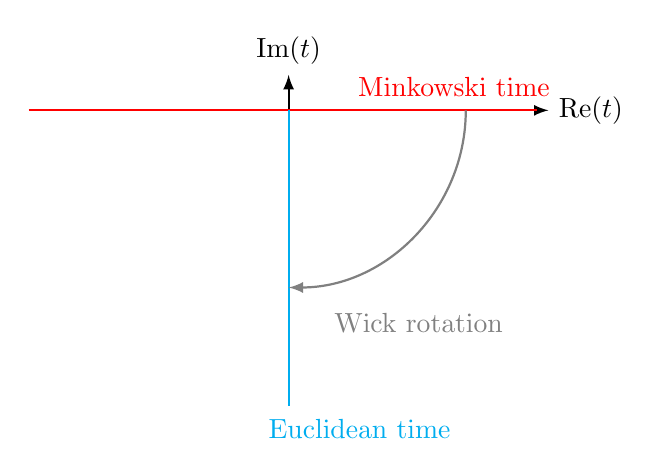
\begin{tikzpicture}[->, thick, scale=1.5]
  % Axes
  \draw[->] (-2.2, 2.5) -- (2.2, 2.5) node[right] {\( \text{Re}(t) \)};
  \draw[->] (0, -0.0) -- (0, 2.8) node[above] {\( \text{Im}(t) \)};
  
  \draw[-,red] (-2.2, 2.5) -- (2.1, 2.5);
  \draw[-,cyan] (0, -0.0) -- (0, 2.5);

  % Arc for Wick rotation
  \draw[->, thick, gray] (1.5, 2.5) arc[start angle=0, end angle=-90, radius=1.5];
  \node at (1.1, 0.7) {\textcolor{gray}{Wick rotation}};
  \node at (0.6, -0.2) {\textcolor{cyan}{Euclidean time}};
  \node at (1.4, 2.7) {\textcolor{red}{Minkowski time}};

\end{tikzpicture}
\end{center}
\end{figure}

\end{itemize}
\end{itemize}

\subsubsection{Path Integral in Quantum Mechanics}
With the simple Hamiltonian
\begin{align}
\hat{H}=\frac{\hat{p}^2}{2m}+V(\hat{q})=K(\hat{q})+V(\hat{q})
\end{align}
we obtain
\begin{align}
e^{-i\hat{H}t}&=e^{-i(\hat{K}+\hat{V})t}\neq e^{-i\hat{K}t}e^{-i\hat{V}t}\\
\lim_{N\rightarrow\infty}\left(e^{-i\hat{H}\frac{t}{N}}\right)^N&=\lim_{N\rightarrow\infty}\left(e^{-i\frac{t}{2N}\hat{V}}e^{-i\frac{t}{N}\hat{K}}e^{-i\frac{t}{2N}\hat{V}}\right)^N\qquad\text{Trotters formula}\\
\rightarrow e^{-i\hat{H}\frac{t}{N}}&=e^{-i\frac{t}{2N}\hat{V}}e^{-i\frac{t}{N}\hat{K}}e^{-i\frac{t}{2N}\hat{V}}e^{\mathcal{O}(1/N^2)}\qquad\text{for large $N$}
\end{align}
With $\tau=t/N$ and
\begin{align}
\hat{T}(\tau)\equiv e^{-i\frac{\tau}{2}\hat{V}}e^{-i\tau\hat{K}}e^{-i\frac{\tau}{2}\hat{V}}=e^{-i\hat{H}\frac{t}{N}}
\end{align}
we can write 
\begin{align}
\langle q^{(f)}|e^{-i\hat{H}t}|q^{(i)}\rangle 
&= \lim_{N\rightarrow\infty} \langle q^{(f)}|\left(\hat{T}(\tau)\right)^N|q^{(i)}\rangle\\
&= \lim_{N\rightarrow\infty} \langle \underbrace{q^{(f)}}_{q^{(N\tau)}}|\underbrace{\hat{T}(\tau)\hat{T}(\tau)\cdots\hat{T}(\tau)\hat{T}(\tau)}_{N-\text{times}}|\underbrace{q^{(i)}}_{q^{(0\tau)}}\rangle
\end{align}
inserting $1=\int d^D q^{(k\tau)}|q^{(k\tau)}\rangle\langle q^{(k\tau)}|$ between all $\hat{T}$
\begin{align}
\langle q^{(f)}|e^{-i\hat{H}t}|q^{(i)}\rangle 
&= \lim_{N\rightarrow\infty}\textcolor{blue}{\int}\cdots\textcolor{red}{\int} \textcolor{blue}{d^Dq^{((N-1)\tau)}}\cdots \textcolor{red}{d^Dq^{(1\tau)}}\\
&\qquad\qquad \langle q^{(N\tau)}|\hat{T}(\tau)\textcolor{blue}{|q^{((N-1)\tau)}\rangle\langle q^{((N-1)\tau)}|}\hat{T}(\tau)\cdots\hat{T}(\tau)\textcolor{red}{|q^{(1\tau)}\rangle\langle q^{(1\tau)}|}\hat{T}(\tau)|q^{(0\tau)}\rangle\\
&=\lim_{N\rightarrow\infty}\int\underbrace{\left[\prod_{n=1}^{N-1}d^Dq^{(n\tau)}\right]}_{\text{lattice path integral measure}}\left[\prod_{k=0}^{N-1}\langle q^{((k+1)\tau)}|\hat{T}(\tau)|q^{(k\tau)}\rangle\right]
\end{align}
Now we investigate the generic transition matrix element
\begin{align}
\langle q'|\hat{T}(\tau)|q\rangle
&=\langle q'|e^{-i\frac{\tau}{2}\hat{V}}e^{-i\tau\hat{K}}e^{-i\frac{\tau}{2}\hat{V}}|q\rangle\\
&=\langle q'|(1-i\frac{\tau}{2}\hat{V}+...)e^{-i\tau\hat{K}}(1-i\frac{\tau}{2}\hat{V}+..)|q\rangle\\
&=(1-i\frac{\tau}{2}V+...)\langle q'|e^{-i\tau\hat{K}}|q\rangle(1-i\frac{\tau}{2}V+..)\\
&\qquad\qquad\qquad\text{with\;} \hat{V}|q\rangle =V(\hat{q})|q\rangle=\sum_k(\partial_q^{(k)}V)\hat{q}^{k}|q\rangle=\sum_k(\partial_q^{(k)}V)q^{k}|q\rangle=V(q)\rangle\\
&=e^{-i\frac{\tau}{2}V(q')}\langle q'|e^{-i\tau\hat{K}}|q\rangle e^{-i\frac{\tau}{2}V(q)}
\end{align}
Now inserting the identity and using the momentum eigenstates
\begin{align}
\langle q'|e^{-i\tau\hat{K}}|q\rangle
&=\int \frac{d^Dp}{(2\pi)^D}\langle q'|p\rangle\langle p|e^{-i\tau\hat{K}}|q\rangle
=\int \frac{d^Dp}{(2\pi)^D}\langle q'|p\rangle\langle p|e^{-i\tau\frac{\hat{p}^2}{2m}}|q\rangle\\
&=\int \frac{d^Dp}{(2\pi)^D}\langle q'|p\rangle e^{-i\tau\frac{p^2}{2m}}\langle p|q\rangle
=\int \frac{d^Dp}{(2\pi)^D}e^{iq'p} e^{-i\tau\frac{p^2}{2m}}e^{-ipq}\\
&=\int \frac{d^Dp}{(2\pi)^D}e^{-i\tau\frac{p^2}{2m}+ip(q'-q)}
=\int \prod_{k=1}^D\frac{dp}{(2\pi)}e^{-i\tau\frac{p_k^2}{2m}+ip_k(q_k'-q_k)}
\end{align}
Solving 1-D integral by completing the square
\begin{align}
\int \frac{dp}{(2\pi)}e^{-i\tau\frac{p^2}{2m}+ip\,\Delta q}
&=\int \frac{dp}{(2\pi)}e^{-\frac{i\tau}{2m}\left(p^2-2\frac{m\,\Delta q}{\tau}p\right)}
=\int \frac{dp}{(2\pi)}e^{-\frac{i\tau}{2m}\left(p^2-2\frac{m\,\Delta q}{\tau}p+\frac{m^2\,\Delta q^2}{\tau^2}-\frac{m^2\,\Delta q^2}{\tau^2}\right)}\\
&=\int \frac{dp}{(2\pi)}e^{-\frac{i\tau}{2m}\left(p^2-\frac{m\,\Delta q}{\tau}\right)^2+\frac{i\tau}{2m}\frac{m^2\,\Delta q^2}{\tau^2}}
=\int \frac{dp}{(2\pi)}e^{-\frac{i\tau}{2m}\left(p^2-\frac{m\,\Delta q}{\tau}\right)^2}e^{i\frac{m\,\Delta q^2}{2\tau}}\\
&=e^{i\frac{m\,\Delta q^2}{2\tau}}\int \frac{d\xi}{(2\pi)}e^{-\frac{\tau}{2m}i\xi^2}
\overset{i\xi^2\rightarrow\zeta^2}{=}e^{i\frac{m\,\Delta q^2}{2\tau}}\int \sqrt{-i}\frac{d\zeta}{(2\pi)}e^{-\frac{\tau}{2m}\zeta^2}\\
&=e^{i\frac{m}{2\tau}\Delta q^2}e^{-i\frac{\pi}{4}}\sqrt{\frac{2m}{\tau}}\sqrt{\pi}\qquad(\text{for\,}\tau>0, t>0)
\end{align}
Then (\textcolor{red}{is there a power of $D$ missing??? - or are we staying in $D=1$})
\begin{align}
\langle q'|\hat{T}(\tau)|q\rangle
&=e^{-i\frac{\tau}{2}V(q')}\langle q'|e^{-i\tau\hat{K}}|q\rangle e^{-i\frac{\tau}{2}V(q)}\\
&=e^{-i\frac{\tau}{2}V(q')}\left(e^{i\frac{m}{2\tau}(q'-q)^2}e^{-i\frac{\pi}{4}}\sqrt{\frac{m}{2\pi\tau}}\textcolor{red}{2\pi}\right) e^{-i\frac{\tau}{2}V(q)}\\
\end{align}
Then collecting all together (with $\partial_s^fq(s)=\frac{q(s+\tau)-q(s)}{\tau}$
\begin{align}
\langle q^{(f)}|e^{-i\hat{H}t}|q^{(i)}\rangle 
&=\lim_{N\rightarrow\infty}\left(e^{-i\frac{\pi}{4}}\sqrt{\frac{m}{2\pi\tau}}\right)^N\int\left[\prod_{n=1}^{N-1}d^Dq^{(n\tau)}\right]
\prod_{k=0}^{N-1}\left[e^{-i\frac{\tau}{2}V(q(s+\tau))}e^{i\frac{m}{2}\tau\frac{(q(s+\tau)-q(s))^2}{\tau^2}}e^{-i\frac{\tau}{2}V(q(s))}\right]_{s=k\tau}\\
&=\lim_{N\rightarrow\infty}\left(e^{-i\frac{\pi}{4}}\sqrt{\frac{m}{2\pi\tau}}\right)^N\int\left[\prod_{n=1}^{N-1}d^Dq^{(n\tau)}\right]
\exp\left[i\tau\sum_{k=0}^{N-1}\frac{m}{2}\frac{(q(s+\tau)-q(s))^2}{\tau^2}-\frac{1}{2}(V(q(s+\tau))+V(q(s)))\right]_{s=k\tau}\\
&=\lim_{N\rightarrow\infty}\left(e^{-i\frac{\pi}{4}}\sqrt{\frac{m}{2\pi\tau}}\right)^N\int\left[\prod_{n=1}^{N-1}d^Dq^{(n\tau)}\right]
\exp\left[i\int_0^t\frac{m}{2}\dot{q}(s)^2-V(q(s))\right]\\
&=\lim_{N\rightarrow\infty}\left(e^{-i\frac{\pi}{4}}\sqrt{\frac{m}{2\pi\tau}}\right)^N\int\left[\prod_{s\in\Lambda_t}d^Dq(s)\right]
\exp\left[iS_M(q)\right]_{q(0)=q^{(i)},q(t)=q^{(f)}}
\end{align}
\begin{itemize}
\item {\bf Exercise 1}: Derive the path-integral formula for
\begin{align}
\langle q^{(f)}|e^{itH}|q^{(i)}\rangle\qquad\text{with\;}t<0
\end{align} 
using the observation
\begin{align}
\langle q^{(f)}|e^{-itH}|q^{(i)}\rangle^*=\langle q^{(f)}|e^{itH}|q^{(i)}\rangle=\langle q^{(f)}|e^{-itH}|q^{(i)}\rangle
\end{align}
\item {\bf Exercise 2}: Calculate
\begin{align}
\langle q'|e^{-\tau\hat{K}}|q\rangle
\end{align} 
\end{itemize}
Euclidean evolution operator $e^{-t\hat{H}}$
\begin{align}
\langle q^{(f)}|e^{-t\hat{H}}|q^{(i)}\rangle
=\lim_{N\rightarrow\infty}\langle q^{(f)}|(\hat{T}(\tau))^N|q^{(i)}\rangle\\
=\lim_{N\rightarrow\infty}\langle q^{(f)}|(e^{-\frac{\tau}{2}\hat{V}}e^{-\tau\hat{K}}e^{-\frac{\tau}{2}\hat{V}})^N|q^{(i)}\rangle
\end{align}
Define effective Hamiltonian ($t=N\tau$)
\begin{align}
\lim_{N\rightarrow\infty}(\hat{T}(\tau))^N&=e^{-t\hat{H}}\\
\hat{T}(\tau)&=e^{-\tau\hat{H}_\text{eff}(\tau)}\\
\rightarrow\hat{H}_\text{eff}(\tau)&=-\frac{1}{\tau}\log\hat{T}(\tau)
\end{align}

\begin{align}
\langle q^{(f)}|e^{-\hat{H}t}|q^{(i)}\rangle 
&=\lim_{N\rightarrow\infty}\left(\sqrt{\frac{m}{2\pi\tau}}\right)^{N\cdot D}\int\left[\prod_{s\in\Lambda_t}d^Dq(s)\right]
\exp\left[-S_E(q)\right]_{q(0)=q^{(i)},q(t)=q^{(f)}}\\
S_E(q)&=\sum_{k=0}^{N-1}\tau\left[\frac{m}{2}|\partial_s^f q(s)|^2+\frac{1}{2}V(q(s))+\frac{1}{2}V(q(s+\tau))\right]_{s=k\tau}
\end{align}

\subsubsection{$\phi^4$-theory}
Hamiltonian and canonical commutation relations are given by ($x=(x_o,\vec{x})$)
\begin{align}
\hat{H}&=\int d^3x\left[\frac{1}{2}\hat{\pi}(\vec{x})^2+\frac{1}{2}\sum_{k=1}^3[\partial_k\hat{\phi}(\vec{x})]^2+\frac{m^2}{2}\hat{\phi}(\vec{x})^2+\frac{\lambda}{4!}\hat{\phi}(\vec{x})^4\right]\\
&[\hat{\phi}(\vec{x}),\hat{\pi}(\vec{x})]=i\delta^{(3)}(\vec{x}-\vec{y})
\end{align}
When we discretize the theory on the lattice we need a $3d$-lattice (because there is NO time in the Hamiltonian or the commutation relations
\begin{align}
\Lambda_s&=a(n_1,n_2,n_3)|\,0\le n_k<N_s\}\\
\hat{H}&=\sum_{\vec{x}\in\Lambda_s}a^3\left[\frac{1}{2}\hat{\pi}(\vec{x})^2+\frac{1}{2}\sum_{k=1}^3[\partial_k^f\hat{\phi}(\vec{x})+\frac{m^2}{2}\hat{\phi}(\vec{x})^2+\frac{\lambda}{4!}\hat{\phi}(\vec{x})^4\right]\\
\partial_k^f\hat{\phi}(\vec{x})&=\frac{\hat{\phi}(\vec{x}+a\hat{e}_k)-\hat{\phi}(\vec{x})}{a}\\
[\hat{\phi}(\vec{x}),\hat{\pi}(\vec{x})]&=ia^{-3}\delta_{\vec{x},\vec{y}}=ia^{-3}\delta_{n_1,m_1}\delta_{n_2,m_2}\delta_{n_3,m_3}\\
\vec{x},\vec{y}&\in\Lambda_s
\end{align}
with $[\hat{\phi}]=\text{mass}^1$,  $[\hat{\pi}]=\text{mass}^2$, $[\delta^{(3)}(\vec{x}-\vec{y})]=\text{mass}^3$. It is sufficient to index $\vec{x}$ with ONE index counter $\vec{x}\simeq x_k$ with $k=1,...,N_s^3$ (and not 3).

In terms of QM - $\phi^4$-theory is a QM point particle in $D=N_s^3$ dimensions in an external potential $V(\hat{\phi})$
\begin{align}
\hat{H}&=\sum_{\vec{x}\in\Lambda_s}\frac{1}{2a^3}\hat{p}(\vec{x})^2+\sum_{\vec{x}\in\Lambda_s}a^3\left[\frac{1}{2}\sum_{k=1}^3[\partial_k^f\hat{\phi}(\vec{x})+\frac{m^2}{2}\hat{\phi}(\vec{x})^2+\frac{\lambda}{4!}\hat{\phi}(\vec{x})^4\right]\\
&=\sum_{\vec{x}\in\Lambda_s}\frac{1}{2a^3}\hat{p}(\vec{x})^2+V(\hat{\phi})\\
\rightarrow\langle\phi^{(f)}|e^{-\hat{H}t}|\phi^{(i)}\rangle
&=\lim_{N_t\rightarrow\infty}\left(\frac{a^3}{2\pi\tau}\right)^{N_tN_s^3/2}\int\prod_{x_0\in\Lambda_t}\prod_{\vec{x}\in\Lambda_s}d\phi(x_o,\vec{x})\; e^{-S_E(\phi)}\\
S_E&=\sum_{k=0}^{N-1}\sum_{\vec{x}\in\Lambda_s}\tau a^3\left\{\frac{1}{2}(\partial_{x_o}^f\phi(\vec{x}))^2+\sum_{\vec{x}\in\Lambda_s}a^3\left[\frac{1}{2}\sum_{k=1}^3[\partial_k^f\phi(\vec{x})]^2+\frac{m^2}{2}\phi(\vec{x})^2+\frac{\lambda}{4!}\phi(\vec{x})^4\right]\right\}_{x_o=k\tau}
\end{align}
Common choice: $a=\tau$ (allowed because eventually we want to take $a,\tau\rightarrow0$). Then for $t>0$
\begin{align}
\langle\phi^{(f)}|e^{-\hat{H}\frac{t}{\tau}}|\phi^{(i)}\rangle
&=\lim_{N_t\rightarrow\infty,\tau=t/N_t}=C_{a,N_s^3 N_t}\int [d\phi]_{(0,t)}e^{-S_{[0,t)}(\phi)}|_{\phi(0,\vec{x})=\phi^{(i)}(\vec{x}),\phi(t,\vec{x})=\phi^{(f)}(\vec{x})}
\end{align}
with
\begin{align}
[d\phi]_{(0,t)}&=\prod_{x_o=\tau}^{t-\tau}\prod_{\vec{x}\in\Lambda_s}d\phi(x_o,\vec{x})\\
S_{[0,t)}(\phi)&=\sum_{x_o=0}^{t-\tau}\tau a^3\left(\frac{1}{2}(\partial_0^f\phi)^2(x)+\frac{V(x)+V(x+\tau\hat{e}_0)}{2}\right)\\
V(x)&=\frac{1}{2}\sum_{k=1}^3(\partial_k^f\phi)^2(x)+\frac{m^2}{2}\phi(x)^2+\frac{\lambda}{4!}\phi(x)^4
\end{align}

\subsubsection{Thermal QFT - QFT in thermodynamic equilibrium}
\begin{itemize}
\item Blackbody radiation = phontons/QED in thermodynamic equilibrium
\item Free energy $F$ of a quantum system in thermal equilirium with temperature $\mathcal{T}$ (with $k_B=1$)
\begin{align}
e^{-\frac{F}{\mathcal{T}}}&=\text{tr}\, e^{-\frac{\hat{H}}{\mathcal{T}}}\\
\rightarrow F&=-\mathcal{T}\log\text{tr}\, e^{-\frac{\hat{H}}{\mathcal{T}}}\\
\rightarrow Z&=\text{tr}\, e^{-\frac{\hat{H}}{\mathcal{T}}}=\text{tr}\, e^{-T\hat{H}}
\end{align}
\end{itemize}
where Euclidean time $T=1/\mathcal{T}$ (inverse temperature)

\subsubsection{Path integral formula for thermal partition function}
\begin{align}
Z(T)
&=\text{tr}\,e^{-T\hat{H}}\\
&=\sum\langle\psi |e^{-T\hat{H}}|\psi\rangle \\
&=\sum\int[\prod_{x\in\Lambda_s}d\phi(\vec{x})]\langle\psi|\phi\rangle\langle\phi|e^{-T\hat{H}}|\psi\rangle\\
&=\int[\prod_{\vec{x}\in\Lambda_s}d\phi(\vec{x})]\langle\phi|e^{-T\hat{H}}|\phi\rangle
\end{align}
discrete version
\begin{align}
Z(T)
&=\text{tr}\,[\hat{T}(\tau)]^{T/\tau}\\
&=\int[\prod_{\vec{x}\in\Lambda_s}d\phi(\vec{x})]\langle\phi|[\hat{T}(\tau)]^{T/\tau}|\phi\rangle\\
&=C_{a,N_tN_s^3}\int[\prod_{\vec{x}\in\Lambda_s}d\phi(\vec{x})][\prod_{x_0=\tau}^{T-\tau}\prod_{x\in\Lambda_s}d\phi(x_0,\vec{x})]e^{-S_{[0,T)}(\phi))}|_{\phi(0,\vec{x})=\phi(T,\vec{x})=\phi(\vec{x})}\\
&=C_{a,N_tN_s^3}\int[\prod_{x_0=0}^{T-\tau}\prod_{x\in\Lambda_s}d\phi(x_0,\vec{x})]e^{-S_{[0,T)}(\phi))}|_{\phi(0,\vec{x})=\phi(T,\vec{x})}
\end{align}
\subsubsection{Thermal time-ordered $n$-point function}
\begin{itemize}
\item {\bf Recall that}: at this point we have 
\begin{itemize}
\item states $|\phi\rangle$
\item operators $\hat{\phi}(\vec{x}), \hat{\pi}(\vec{x}), \hat{H}$
\end{itemize} 
which do NOT depend on time 
\item and then we have the evolution operator $e^{-itH}$ or $e^{-tH}$
\item {\bf NOW:} operators in Heisenberg representation (time dependence get attached to the operator)
\begin{itemize}
\item Minkowskian
\begin{align}
\hat{O}(t)&=e^{i\hat{H}t}\hat{O}e^{-i\hat{H}t}\\
\hat{\phi}(x_0,\vec{x})&=e^{i\hat{H}x_0}\hat{\phi}(\vec{x})e^{-i\hat{H}x_0}
\end{align}
\item Euclidean
\begin{align}
\hat{O}(t)&=e^{\hat{H}t}\hat{O}e^{-\hat{H}t}\\
\hat{\phi}(x_0,\vec{x})&=e^{\hat{H}x_0}\hat{\phi}(\vec{x})e^{i\hat{H}x_0}
\end{align}
\end{itemize}

\end{itemize}

\newpage
\begin{enumerate}
\item Lowest energy levels can be extracted from from the exponential decay of the connected (vacuum) 2-point functions in Euclidean time - In practise this method is used to extract masses in lattice simulations
\item Energy levels are poles in the complex $p_0$-plane of connected 2-point functions (in momentum space) 
\end{enumerate}

\newpage
\subsubsection{Free scalar theory}
\begin{itemize}
\item Discretized action (with periodic boundary conditions)
\begin{align}
S&=\sum_x a^4\left\{\frac{1}{2}\sum_\mu\partial_\mu^f\phi(x)\partial_\mu^f\phi(x)+\frac{m^2}{2}\phi(x)^2\right\}\\
Z(0)&=\int_\mathcal{C}d\phi\,e^{-S}\\
\langle\phi(x_1)...\phi(x_n)\rangle&=\frac{1}{Z}\int_\mathcal{C}d\phi\,e^{-S}\phi(x_1)...\phi(x_n)
\end{align}
on configuration space $\mathcal{C}=\mathbb{R}^{N_t\cdot N_s^3}$.
\item 1 dimension ($\oplus\equiv$ sum modulo $Na$ )
\begin{align}
\sum_{x/a=0}^{N-1}\partial_1^f\phi(x)\chi(x)
&=\sum_{x/a=0}^{N-1}\frac{\phi(x\oplus a)-\phi(x)}{a}\chi(x)\\
&=\frac{1}{a}\sum_{x/a=0}^{N-1}\phi(x\oplus a)\chi(x)-\frac{1}{a}\sum_{x/a=0}^{N-1}\phi(x)\chi(x)\\
&\overset{x\rightarrow x\ominus a}{=}\frac{1}{a}\sum_{x/a=1}^{N}\phi(x)\chi(x\ominus a)-\frac{1}{a}\sum_{x/a=0}^{N-1}\phi(x)\chi(x)\\
&=\sum_{x/a=1}^{N-1}\phi(x)\frac{\chi(x\oplus a)-\chi(x)}{a}\\
&=-\sum_{x/a=0}^{N-1}\phi(x)\partial_1^b\chi(x)
\end{align}
or in short with $(\phi,\chi)\equiv\sum_x\phi(x)\chi(x)$
\begin{align}
(\partial_\mu^f\phi,\chi)&=-(\phi,\partial_\mu^b\chi)\\
\rightarrow (\partial_\mu^f)^\dagger&=-\partial_\mu^b
\end{align}
\item Then we can rewrite the action as (using the discretized Laplacian $\hat{\Box}=\sum_\mu\partial_\mu^b\partial_\mu^f$)
\begin{align}
S
&=\frac{a^4}{2}\sum_\mu(\partial_\mu^f\phi,\partial_\mu^f\phi)+\frac{m^2a^4}{2}(\phi,\phi)\\
&=\frac{a^4}{2}\sum_\mu(\phi,-\partial_\mu^b\partial_\mu^f\phi)+\frac{m^2a^4}{2}(\phi,\phi)\\
&=\frac{a^4}{2}\sum_\mu(\phi,-\hat{\Box}\phi)+\frac{m^2a^4}{2}(\phi,\phi)\\
&=\frac{a^4}{2}\sum_\mu(\phi,(-\hat{\Box}+m^2)\phi)
\end{align}
\item Define a generating functional
\begin{align}
Z(J)=\int_\mathcal{C}d\phi\,e^{-S+\sum_x a^4J(x)\phi(x)}
\end{align}
and using the result of exercise 2 (sheet 1)
\begin{align}
Z(J)&=\int d\phi e^{-\frac{1}{2}(\phi,A\phi)+(a^4 J,\phi)}=\frac{(2\pi)^{N_tN_s^3/2}}{\sqrt{\det{A}}}e^{\frac{1}{2}(a^4J,A^{-1}a^4J)}\\
&\rightarrow A=a^4(-\hat{\Box}+m^2)
\end{align}
we obtain
\begin{align}
Z(J)=\left(\frac{2\pi}{a^4}\right)^{N_t N_s^3/2}\frac{1}{\sqrt{\det(-\hat{\Box}+m^2)}}e^{\frac{a^4}{2}\left(J,(-\hat{\Box}+m^2)^{-1}J\right)}
\end{align}
\item and therefore
\begin{align}
\langle\phi(x_1)...\phi(x_n)\rangle
&=\left.\frac{1}{Z(J)}\frac{1}{a^4}\frac{\partial}{\partial J(x_1)}...\frac{1}{a^4}\frac{\partial}{\partial J(x_n)}Z(J)\right|_{J=0}\\
&=\left.\frac{1}{a^4}\frac{\partial}{\partial J(x_1)}...\frac{1}{a^4}\frac{\partial}{\partial J(x_n)}e^{\frac{a^4}{2}\left(J,(-\hat{\Box}+m^2)^{-1}J\right)}\right|_{J=0}\\
&=\left.\frac{1}{a^4}\frac{\partial}{\partial J(x_1)}...\frac{1}{a^4}\frac{\partial}{\partial J(x_n)}e^{\frac{a^4}{2}\sum_{xy}J(x)(-\hat{\Box}+m^2)^{-1}(x,y)J(y)}\right|_{J=0}\\
\rightarrow\langle\phi(x)...\phi(y)\rangle
&=\left.\frac{1}{a^4}\frac{\partial}{\partial J(x)}\frac{1}{a^4}\frac{\partial}{\partial J(y)}e^{\frac{a^4}{2}\sum_{xy}J(x)(-\hat{\Box}+m^2)^{-1}(x,y)J(y)}\right|_{J=0}\\
&=...\\
&=\frac{1}{a^4}(-\hat{\Box}+m^2)^{-1}(x,y)
\end{align}
\item Observation: We can diagonalize $(-\hat{\Box}+m^2)$ meaning we can express it in terms of 
\begin{itemize}
\item eigenvectors: plane waves $\psi_p(x)=e^{ixp}$ with periodic boundary conditions
\begin{align}
\psi_p(x+aN_te_0)&=\psi_p(x)\quad\rightarrow\quad e^{iaN_tp_0}=1\quad\rightarrow\quad p_0=\frac{2\pi}{aN_t}\mathbb{Z}\\
\psi_p(x+aN_se_k)&=\psi_p(x)\quad\rightarrow\quad e^{iaN_sp_k}=1\quad\rightarrow\quad p_k=\frac{2\pi}{aN_t}\mathbb{Z}
\end{align}
\item eigenvalues
\end{itemize}
\item $\hat{\Box}$ is a $N_tN_s^3\times N_tN_s^3$ matrix with $N_tN_s^3$ independent eigenvectors
\begin{align}
\psi_p&=e^{i(p+\frac{2\pi}{a}e_\mu)x}\\
p&=\left(\frac{2\pi}{aN_t}k_0,\frac{2\pi}{aN_s}k_1,\frac{2\pi}{aN_s}k_2,\frac{2\pi}{aN_s}k_3\right)\qquad k_\mu\in\mathbb{Z}\\
&\rightarrow -\frac{\pi}{a}<p_\mu\le\frac{\pi}{a}
\end{align}
so there are $N_tN_s^3$ possible values of momenta
\item then
\begin{align}
(\psi_p,\psi_{p'})
&=\sum_x(e^{ixp})^*(e^{ixp'})
=\sum_xe^{ix(p'-p)}\\
&=\sum_xe^{i\sum_\mu x_\mu(p_\mu'-p_\mu)}
=\prod_\mu\sum_{x_\mu/a=0}^{N_\mu-1}e^{i \frac{x_\mu}{a}a(p_\mu'-p_\mu)}\\
&=...
=N_tN_s^3\delta_{pp'}
\end{align}
\item and
\begin{align}
\hat{\Box}\psi_p(x)
&=\sum_\mu\partial_\mu^b\partial_\mu^f\psi_p(x)\\
&=\sum_\mu\frac{\psi_p(x\oplus ae_\mu)+\psi_p(x\ominus ae_\mu-2\psi_p(x))}{a^2}
=\sum_\mu\frac{e^{ip(x+ae_\mu)}+e^{ip(x-ae_\mu)}-2e^{ipx}}{a^2}\\
&=\psi_p(x)\sum_\mu\frac{e^{iap_\mu}+e^{-iap_\mu}-2}{a^2}
=\psi_p(x)\sum_\mu\frac{(e^{iap_\mu}-e^{-iap_\mu})^2}{a^2}\\
&=\psi_p(x)\sum_\mu\frac{(2i\sin(ap_\mu/2))^2}{a^2}
=-\psi_p(x)\sum_\mu\frac{4}{a^2}\sin^2\frac{ap_\mu}{2}\\
&\overset{a\rightarrow0}{\rightarrow}-\psi_p\sum_\mu\frac{4}{a^2}\left(\frac{ap_\mu}{2}\right)^2
=-\psi_p\sum_\mu p_\mu^2
\end{align}
\item Using completeness relation regarding the orthonormal basis of eigenvectors  $\{\psi_p/\sqrt{N_tN_s^3}\}$
\begin{align}
(-\hat{\Box}+m^2)^{-1}
&=(-\hat{\Box}+m^2)^{-1}I\\
&=(-\hat{\Box}+m^2)^{-1}\sum_p\frac{\psi_p}{\sqrt{N_tN_s^3}}\frac{\psi_p^\dagger}{\sqrt{N_tN_s^3}}\\
&=\frac{1}{N_tN_s^3}\sum_p\frac{\psi_p\psi_p^\dagger}{\sum_\mu\frac{4}{a^2}\sin^2\frac{ap_\mu}{2}+m^2}\\
(-\hat{\Box}+m^2)^{-1}(x,y)
&=\frac{1}{N_tN_s^3}\sum_p\frac{e^{ip(x-y)}}{\sum_\mu\frac{4}{a^2}\sin^2\frac{ap_\mu}{2}+m^2}
\end{align}
this means the 2-point function can be written as
\begin{align}
\rightarrow\langle\phi(x)...\phi(y)\rangle
&=\frac{1}{a^4}(-\hat{\Box}+m^2)^{-1}(x,y)\\
&=\frac{1}{TL^3}\sum_p\frac{e^{ip(x-y)}}{\sum_\mu\frac{4}{a^2}\sin^2\frac{ap_\mu}{2}+m^2}
\end{align}
\item {\bf Exercise 1}: Calculate the $T\rightarrow\infty$ limit of $\langle\phi(x)...\phi(y)\rangle$ (this is related to the vacuum expectation value of the product of two fields)
\item {\bf Exercise 2}: Go to momentum space in the temporal coordinate (i.e you can set $y=0$, $x_0\rightarrow p_0$)
\item {\bf Exercise 3}: Find the poles in the complex $p_0$ place and check that they have the general structure discussed in the previous lecture (in particular, write energy levels)
\end{itemize}

\subsection{Scalar QED}
Complex scalar field $\phi(x)\in\mathbb{C}$ and real 4-component photon field $A_\mu(x)\in\mathbb{R}$
\begin{align}
S&=\int d^4x\left\{\frac{1}{4e^2}F_{\mu\nu}^2+\sum+\mu|D_\mu\phi|^2+m^2|\phi|^2+\frac{\lambda}{4}|\phi|^4\right\}\\
F_{\mu\nu}&=\partial_\mu A_\nu-\partial_\nu A_\mu\\
D_\mu&=\partial_\mu+iA_\mu
\end{align}
Gauge symmetry
\begin{align}
\phi(x)&\rightarrow e^{i\alpha(x)}\phi(x)\\
\phi(x)^\dagger&\rightarrow e^{-i\alpha(x)}\phi(x)^\dagger\\
A_\mu(x)&\rightarrow A_\mu(x)-\partial_\mu\alpha(x)\\
D_\mu\phi(x)&=\partial_\mu\phi+iA_\mu(x)\phi(x)\\
&\rightarrow\partial_\mu
\left(e^{i\alpha(x)}\phi(x)\right)
+i\left(A_\mu(x)-\partial_\mu\alpha(x)\right)
e^{i\alpha(x)}\phi(x)\\
&\rightarrow e^{i\alpha(x)}D_\mu\phi(x)\\
F_{\mu\nu}&\rightarrow\partial_\mu(A_\nu-\partial_\nu\alpha)-\partial_\nu(A_\mu-\partial_\mu\alpha)\\
&\rightarrow F_{\mu\nu}
\end{align}
\begin{itemize}
\item If you just replace $\partial_\mu\rightarrow\partial_\mu^f$ and $\int d^4x\rightarrow\sum_xa^4$ - then $S$ is NOT gauge invariant 
\begin{align}
D_\mu\phi(x)
&\simeq\partial_\mu^f\phi(x)+iA_\mu(x)\phi(x)\\
&\simeq\frac{1}{a}(\phi(x+ae_\mu)-\phi(x))+iA_\mu(x)\phi(x)\\
&\rightarrow\frac{1}{a}(e^{i\alpha(x+ae_\mu)}\phi(x+ae_\mu)-e^{i\alpha(x)}\phi(x))+iA'_\mu(x)e^{i\alpha(x)}\phi(x)\\
&\quad\overset{!}{=}e^{i\alpha(x)}D_\mu\phi(x)\\
&\quad=e^{i\alpha(x)}\left(\frac{1}{a}(\phi(x+ae_\mu)-\phi(x))+iA_\mu(x)\phi(x)\right)\\
\rightarrow A'_\mu(x)&=A_\mu(x)+\frac{1}{a}\left(e^{i\alpha(x)}-e^{i\alpha(x+ae_\mu)}\right)\frac{\phi(x+ae_\mu)}{ie^{i\alpha(x)}\phi(x)}
\end{align}
we see that requiring gauge covariance of the (naively discretized) $D_\mu\phi(x)$ implies that the gauge transformation of $A_\mu(x)$ depends on the matter field ${\bf \textcolor{red}{\rightarrow FAIL!}}$ 

\item Guiding principle: find a discretization that preserves gauge invariance
\item We want to find a formulation in which gauge fixing is not needed at all (as long as we don't care about perturbative expansions)
\end{itemize}
When (parallel) transport $\phi(x+ae_\mu)$ back to point $x$ using the parallel transporter (which makes only sense in a continuum)
\begin{align}
e^{i\int_0^a ds\, A_\mu(\textcolor{blue}{x+se_\mu})}\phi(x+ae_\mu)
&\overset{\text{gauge}}{\rightarrow} e^{i\int_0^a ds\, [A_\mu(\textcolor{blue}{x+se_\mu})-\partial_\mu\alpha(x+se_\mu)]}e^{i\alpha(x+ae_\mu)}\phi(x+ae_\mu)\\
&\rightarrow e^{i\int_0^a ds\, A_\mu(\textcolor{blue}{x+se_\mu})}\underbrace{e^{-i\int_0^a ds\,\partial_\mu\alpha(x+se_\mu)}}_{=e^{-i(\alpha(x+ae_\mu)-\alpha(x))}}e^{i\alpha(x+ae_\mu)}\phi(x+ae_\mu)\\
&\rightarrow e^{i\int_0^a ds\, A_\mu(\textcolor{blue}{x+se_\mu})}e^{i\alpha(x)}\phi(x+ae_\mu)\\
&\rightarrow e^{i\alpha(x)}\,\left[e^{i\int_0^a ds\, A_\mu(\textcolor{blue}{x+se_\mu})}\phi(x+ae_\mu)\right]
\end{align}
the object transforms under a gauge transform like $\phi(x)$. Then we define
\begin{align}
D_\mu^f(x)
&\equiv\frac{[\text{parallel transported}\,\phi(x+ae_\mu)]-\phi(x) }{a}\\
&=\frac{e^{i\int_0^a ds\, A_\mu(x+se_\mu)}\phi(x+ae_\mu)-\phi(x) }{a}\\
\end{align}
with properties
\begin{enumerate}[(1)]
\item $D_\mu^f\phi(x)\overset{\text{gauge}}{\rightarrow}e^{i\alpha(x)}D_\mu^f\phi(x)$ (see above)
\item $\lim_{a\rightarrow0}D_\mu^f\phi(x)=D_\mu\phi(x)=[\partial_\mu+iA_\mu(x)]\phi(x)$
\end{enumerate}
Proof of (2)
\begin{align}
\int_0^a ds\,A_\mu(x+se_\mu)&\simeq\int_0^a\left(A_\mu(x)+\mathcal{O}(s)\right)\\
&=aA_\mu(x)+\mathcal{O}(a^2)\\
\rightarrow \lim_{a\rightarrow0}D_\mu^f\phi(x)
&=\lim_{a\rightarrow0}\frac{e^{i\int_0^a ds\, A_\mu(x+se_\mu)}\phi(x+ae_\mu)-\phi(x)}{a}\\
&=\lim_{a\rightarrow0}\frac{e^{iaA_\mu(x)+\mathcal{O}(a^2)}[\phi(x)+a\partial_\mu\phi(x)+\mathcal{O}(a^2)]-\phi(x)}{a}\\
&=\lim_{a\rightarrow0}\frac{(1+iaA_\mu(x)+\mathcal{O}(a^2))[\phi(x)+a\partial_\mu\phi(x)+\mathcal{O}(a^2)]-\phi(x)}{a}\\
&=\lim_{a\rightarrow0}\frac{(\phi(x)+iaA_\mu(x)\phi(x))+(a\partial_\mu\phi(x)+iaA_\mu(x)a\partial_\mu\phi(x))-\phi(x)}{a}\\
&=\lim_{a\rightarrow0}\frac{(iaA_\mu(x)\phi(x))+a\partial_\mu\phi(x)}{a}\\
&=\partial_\mu\phi(x)+iA_\mu(x)\phi(x))\\
&=D_\mu\phi(x)
\end{align}
On the lattice we will only need to transport matter fields form one lattice point to another lattice point. Therefore we do not need the field $A_\mu(x)$ but only the parallel transporters
\begin{align}
W(x\rightarrow x+ae_\mu)
&\equiv U_\mu(x)\\
&\equiv e^{i\int_0^a ds\,A_\mu(x+se_\mu)}\in U(1)
\end{align}
\begin{itemize}
\item {\bf Important: } $U_\mu(x)$ are going to be the fundamental degrees of freedom that describes the gauge field on the lattice and \textcolor{red}{\bf NOT} $A_\mu(x)$
\item These transformations ensure that the terms of the actions containing a matter field are gauge invariant. 
\item What about $F_{\mu\nu}^2$?
\begin{itemize}
\item We need to find a discretization of $F_{\mu\nu}^2$ that depends only on $U_\mu(x)$ and not on $A_\mu(x)$
\item $F_{\mu\nu}^2$ can be written in terms of the parallel transports on the smallest squares on the lattice
\begin{center}
\begin{figure}[!h]
\centering
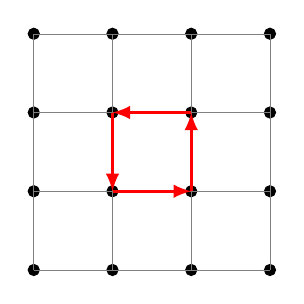
\begin{tikzpicture}
\def\L{3}
  % Draw the lattice points in a 5x5 grid
  \foreach \x in {0,...,\L}
    \foreach \y in {0,...,\L}
      \filldraw[black] (\x,\y) circle (2pt);
  
  % Optional: draw a grid
  \draw[step=1cm, gray, very thin] (0,0) grid (\L,\L);
  \draw[->, red, very thick] (1,1) -- (2,1) node[midway, left]  {};
  \draw[->, red, very thick] (2,1) -- (2,2) node[midway, left]  {};
  \draw[->, red, very thick] (2,2) -- (1,2) node[midway, left]  {};
  \draw[->, red, very thick] (1,2) -- (1,1) node[midway, left]  {};
\end{tikzpicture}
\end{figure}
\end{center}

\end{itemize}
\begin{align}
S[U,\phi]=\sum_{x_\mu}a^4\left\{?+|D_\mu\phi|^2+m^2|\phi|^2+\frac{\lambda_0}{4}|\phi|^4\right\}
\end{align}




\end{itemize}


\end{document}